% Judul dokumen
\title{Buku Tugas Akhir ITS}
\author{Hariyantoputera, Rifqi Alhakim}

% Pengaturan ukuran teks dan bentuk halaman dua sisi
\documentclass[12pt,twoside]{report}

% Pengaturan ukuran halaman dan margin
\usepackage[a4paper,top=30mm,left=30mm,right=20mm,bottom=25mm]{geometry}

% Pengaturan ukuran spasi
\usepackage[singlespacing]{setspace}

% Pengaturan format bahasa
\usepackage[indonesian]{babel}

% Pengaturan detail pada file PDF
\usepackage[pdfauthor={\@author},bookmarksnumbered,pdfborder={0 0 0}]{hyperref}

% Pengaturan jenis karakter
\usepackage[utf8]{inputenc}

% Pengaturan pewarnaan
\usepackage[table,xcdraw]{xcolor}

% Pengaturan kutipan artikel
\usepackage[numbers]{natbib}

% Package lainnya
\usepackage{changepage}
\usepackage{enumitem}
\usepackage{eso-pic}
\usepackage{etoolbox}
\usepackage{graphicx}
\usepackage{lipsum}
\usepackage{lmodern}
\usepackage{longtable}
\usepackage{tabularx}
\usepackage{wrapfig}
\usepackage{float}

% Definisi untuk "Hati ini sengaja dikosongkan"
\patchcmd{\cleardoublepage}{\hbox{}}{
  \thispagestyle{empty}
  \vspace*{\fill}
  \begin{center}\textit{[Halaman ini sengaja dikosongkan]}\end{center}
  \vfill}{}{}

% Pengaturan penomoran halaman
\usepackage{fancyhdr}
\fancyhf{}
\renewcommand{\headrulewidth}{0pt}
\pagestyle{fancy}
\fancyfoot[RE,RO]{\thepage}
\patchcmd{\chapter}{plain}{fancy}{}{}
\patchcmd{\chapter}{empty}{plain}{}{}

% Pengaturan format judul bab
\usepackage{titlesec}
\titleformat{\chapter}[display]{\bfseries\Large}{BAB \centering\Roman{chapter}}{0ex}{\vspace{0ex}\centering}
\titleformat{\section}{\bfseries\large}{\MakeUppercase{\thesection}}{1ex}{\vspace{1ex}}
\titleformat{\subsection}{\bfseries\large}{\MakeUppercase{\thesubsection}}{1ex}{}
\titleformat{\subsubsection}{\bfseries\large}{\MakeUppercase{\thesubsubsection}}{1ex}{}
\titlespacing{\chapter}{0ex}{0ex}{4ex}
\titlespacing{\section}{0ex}{1ex}{0ex}
\titlespacing{\subsection}{0ex}{0.5ex}{0ex}
\titlespacing{\subsubsection}{0ex}{0.5ex}{0ex}

% Pengaturan format potongan kode
\usepackage{listings}
\definecolor{comment}{RGB}{0,128,0}
\definecolor{string}{RGB}{255,0,0}
\definecolor{keyword}{RGB}{0,0,255}
\lstdefinestyle{codestyle}{
  commentstyle=\color{comment},
  stringstyle=\color{string},
  keywordstyle=\color{keyword},
  basicstyle=\footnotesize\ttfamily,
  numbers=left,
  numberstyle=\tiny,
  numbersep=5pt,
  frame=lines,
  breaklines=true,
  prebreak=\raisebox{0ex}[0ex][0ex]{\ensuremath{\hookleftarrow}},
  showstringspaces=false,
  upquote=true,
  tabsize=2,
}
\lstset{style=codestyle}

% Isi keseluruhan dokumen
\begin{document}

  % Sampul luar Bahasa Indonesia
  \newcommand\covercontents{sampul/konten-id.tex}
  \AddToShipoutPictureBG*{
  \AtPageLowerLeft{
    % Ubah nilai berikut jika posisi horizontal background tidak sesuai
    \hspace{-3.5mm}

    % Ubah nilai berikut jika posisi vertikal background tidak sesuai
    \raisebox{0mm}{
      
\includegraphics[width=\paperwidth,height=\paperheight]{sampul/gambar/sampul-luar2.png}
    }
  }
}

% Menyembunyikan nomor halaman
\thispagestyle{empty}

% Pengaturan margin untuk menyesuaikan konten sampul
\newgeometry{
  top=55mm,
  left=30mm,
  right=20mm,
  bottom=25mm
}

\begin{flushleft}
  % Pemilihan font sans serif
  \sffamily

  % Pemilihan warna font putih
  \color{white}

  % Pemilihan font bold
  % \fontseries{bx}
  \selectfont

  \input{\covercontents}

\end{flushleft}

\restoregeometry


  % Atur ulang penomoran halaman
  \setcounter{page}{1}

  % Sampul dalam Bahasa Indonesia
  \renewcommand\covercontents{sampul/konten-id.tex}
  \AddToShipoutPictureBG*{
  \AtPageLowerLeft{
    % Ubah nilai berikut jika posisi horizontal background tidak sesuai
    \hspace{-3.5mm}

    % Ubah nilai berikut jika posisi vertikal background tidak sesuai
    \raisebox{0mm}{
      
\includegraphics[width=\paperwidth,height=\paperheight]{sampul/gambar/sampul-dalam2.png}
    }
  }
}

% Menyembunyikan nomor halaman
\thispagestyle{empty}

% Pengaturan margin untuk menyesuaikan konten sampul
\newgeometry{
  top=65mm,
  left=30mm,
  right=20mm,
  bottom=25mm
}

\begin{flushleft}

  % Pemilihan font sans serif
  \sffamily

  % Pemilihan font bold
  % \fontseries{bx}
  \selectfont

  \input{\covercontents}

\end{flushleft}

\restoregeometry

  \clearpage
  \cleardoublepage

  % Sampul dalam Bahasa Inggris
  \renewcommand\covercontents{sampul/konten-en.tex}
  \AddToShipoutPictureBG*{
  \AtPageLowerLeft{
    % Ubah nilai berikut jika posisi horizontal background tidak sesuai
    \hspace{-3.5mm}

    % Ubah nilai berikut jika posisi vertikal background tidak sesuai
    \raisebox{0mm}{
      
\includegraphics[width=\paperwidth,height=\paperheight]{sampul/gambar/sampul-dalam2.png}
    }
  }
}

% Menyembunyikan nomor halaman
\thispagestyle{empty}

% Pengaturan margin untuk menyesuaikan konten sampul
\newgeometry{
  top=65mm,
  left=30mm,
  right=20mm,
  bottom=25mm
}

\begin{flushleft}

  % Pemilihan font sans serif
  \sffamily

  % Pemilihan font bold
  % \fontseries{bx}
  \selectfont

  \input{\covercontents}

\end{flushleft}

\restoregeometry

  \cleardoublepage

  % Pengaturan ukuran indentasi paragraf
  \setlength{\parindent}{2em}

  % Pengaturan ukuran spasi paragraf
  \setlength{\parskip}{1ex}

  % Lembar pengesahan
  \begin{center}
	\large
  \textbf{LEMBAR PENGESAHAN}
\end{center}

% Menyembunyikan nomor halaman
\thispagestyle{empty}

\begin{center}
  % Ubah kalimat berikut dengan judul tugas akhir
  \textbf{\emph{SMART WHITEBOARD:} PENGENALAN TEKS HURUF BALOK MENGGUNAKAN \emph{YOU ONLY LOOK ONCE (YOLO)}}
\end{center}

\begingroup
  % Pemilihan font ukuran small
  \small
  
  \vspace{3ex}

  \begin{center}
    \textbf{PROPOSAL TUGAS AKHIR}
    \\Diajukan untuk memenuhi salah satu syarat
    \\memperoleh gelar Sarjana pada
    \\Program Studi S-1 Teknik Komputer
    \\Departemen Teknik Komputer
    \\Fakultas Teknologi Elektro dan Informatika Cerdas
    \\Institut Teknologi Sepuluh Nopember
  \end{center}

  \vspace{3ex}

  \begin{center}
    % Ubah kalimat berikut dengan nama dan NRP mahasiswa
    Oleh: Rifqi Alhakim Hariyantoputera 
    \\NRP. 0721 18 4000 0055
  \end{center}

  \vspace{3ex}

  % \begin{center}
  % Ubah kalimat-kalimat berikut dengan tanggal ujian dan periode wisuda
  %   Tanggal Ujian : 1 Juni 2021\\
  %   Periode Wisuda : September 2021
  % \end{center}

  \begin{center}
    Disetujui oleh Tim Penguji Tugas Akhir:
  \end{center}

  \vspace{4ex}

  \begingroup
    % Menghilangkan padding
    \setlength{\tabcolsep}{0pt}

    \noindent
    \begin{tabularx}{\textwidth}{X l}
      % Ubah kalimat-kalimat berikut dengan nama dosen pembimbing pertama
      1. Dr. Eko Mulyanto Yuniarno, S.T., M.T.          & Pembimbing \\
      % NIP: 18560710 194301 1 001        & ................................... \\
      &  \\
      &  \\
      % Ubah kalimat-kalimat berikut dengan nama dosen pembimbing kedua
      2. Reza Fuad Rachmadi, S.T., M.T., Ph.D.     & Ko-Pembimbing \\
      &  \\
      &  \\
      % Ubah kalimat-kalimat berikut dengan nama dosen penguji pertama
      3. Dr. Galileo Galilei, S.T., M.Sc.  & Penguji I \\
      &  \\
      &  \\
      % Ubah kalimat-kalimat berikut dengan nama dosen penguji kedua
      4. Friedrich Nietzsche, S.T., M.Sc.  & Penguji II \\
      &  \\
      &  \\
      % Ubah kalimat-kalimat berikut dengan nama dosen penguji ketiga
      5. Alan Turing, ST., MT.             & Penguji III \\
      &  \\
      &  \\
    \end{tabularx}
  \endgroup

  \vspace{12ex}

  % \begin{center}
  %   % Ubah kalimat berikut dengan jabatan kepala departemen
  %   Mengetahui, \\
  %   Kepala Departemen Teknik Dirgantara FTD - ITS \\

  %   \vspace{8ex}

  %   % Ubah kalimat-kalimat berikut dengan nama dan NIP kepala departemen
  %   \underline{Dr. Leonardo Da Vinci, S.T., M.T.} \\
  %   NIP. 14520415 151905 1 001
  % \end{center}

  \begin{center}
    \textbf{SURABAYA\\Bulan, 2022}
  \end{center}
\endgroup

  \cleardoublepage

  % Pernyataan keaslian
  \begin{center}
  \large
  \textbf{PERNYATAAN ORISINALITAS}
\end{center}

% Menyembunyikan nomor halaman
\thispagestyle{empty}

\vspace{2ex}

% Ubah paragraf-paragraf berikut sesuai dengan yang ingin diisi pada pernyataan keaslian

\noindent Yang bertanda tangan dibawah ini:

\noindent\begin{tabularx}{\textwidth}{X X l}
  & \\
  Nama Mahasiswa / NRP &: Elon Reeve Musk / 0123 20 4000 0001 \\
  Departemen &: Departemen \\
  Dosen Pembimbing &: Nama Dosen Pembimbing \\
  & \\
\end{tabularx}

Dengan ini menyatakan bahwa Tugas Akhir dengan judul "" adalah hasil karya sendiri, berfsifat orisinal, dan ditulis dengan mengikuti kaidah penulisan ilmiah.

Bilamana di kemudian hari ditemukan ketidaksesuaian dengan pernyataan ini, maka saya bersedia menerima sanksi sesuai dengan ketentuan yang berlaku di Institut Teknologi Sepuluh Nopember.

\vspace{8ex}

\noindent\begin{tabularx}{\textwidth}{X l}
  % Ubah kalimat berikut sesuai dengan tempat, bulan, dan tahun penulisan
  & Surabaya, Mei 2021\\
  & \\
  Mengetahui & \\
  Dosen Pembimbing & Mahasiswa\\
  & \\
  & \\
  & \\
  & \\
  & \\
  (Nama Dosen Pembimbing) & (Nama Mahasiswa) \\
  NIP. & NRP. \\
\end{tabularx}
  \cleardoublepage

  % Nomor halaman pembuka dimulai dari sini
  \pagenumbering{roman}

  % Abstrak Bahasa Indonesia
  \begin{center}
  \large\textbf{ABSTRAK}
\end{center}

\addcontentsline{toc}{chapter}{ABSTRAK}

\vspace{2ex}

\begingroup
  % Menghilangkan padding
  \setlength{\tabcolsep}{0pt}

  \noindent
  \begin{tabularx}{\textwidth}{l >{\centering}m{2em} X}
    % Ubah kalimat berikut dengan nama mahasiswa
    Nama Mahasiswa    &:& Elon Reeve Musk \\

    % Ubah kalimat berikut dengan judul tugas akhir
    Judul Tugas Akhir &:&	Kalkulasi Energi pada Roket Luar Angkasa Berbasis \emph{Anti-Gravitasi} \\

    % Ubah kalimat-kalimat berikut dengan nama-nama dosen pembimbing
    Pembimbing        &:& 1. Nikola Tesla, S.T., M.T. \\
                      & & 2. Wernher von Braun, S.T., M.T. \\
  \end{tabularx}
\endgroup

% Ubah paragraf berikut dengan abstrak dari tugas akhir
Pada penelitian ini kami mengajukan \lipsum[1]

% Ubah kata-kata berikut dengan kata kunci dari tugas akhir
Kata Kunci: Roket, \emph{Anti-gravitasi}, Energi, Angkasa.

  \cleardoublepage

  % Abstrak Bahasa Inggris
  \begin{center}
  \large\textbf{ABSTRACT}
\end{center}

\addcontentsline{toc}{chapter}{ABSTRACT}

\vspace{2ex}

\begingroup
  % Menghilangkan padding
  \setlength{\tabcolsep}{0pt}

  \noindent
  \begin{tabularx}{\textwidth}{l >{\centering}m{3em} X}
    % Ubah kalimat berikut dengan nama mahasiswa
    \emph{Name}     &:& Rifqi Alhakim Hariyantoputera \\

    % Ubah kalimat berikut dengan judul tugas akhir dalam Bahasa Inggris
    \emph{Title}    &:& \emph{Uppercase Letter Detection On Whiteboard Using You Only Look Once (YOLO)} \\

    % Ubah kalimat-kalimat berikut dengan nama-nama dosen pembimbing
    \textit{Advisor}  &:& 1. Dr. Eko Mulyanto Yuniarno, S.T., M.T. \\
                      & & 2. Reza Fuad Rachmadi, S.T., M.T., Ph.D. \\
  \end{tabularx}
\endgroup

% Ubah paragraf berikut dengan abstrak dari tugas akhir dalam Bahasa Inggris
\textit{Communication is a process where a person or persons, groups, organizations, or communities create and use information to connect with the environment and other people. Writing is a form of communication. With writing, an idea can be poured and conveyed to other parties without having to be in the same place with other parties, and an idea can be immortalized. 
In order to understand a document, segmentation of image documents into a sentence form is an important step to understand a document. Unlike printed documents which already have a certain format in their writing, handwritten documents have very much variations. Technological development innovation applied to the blackboard is an effort to increase the role of technology in education sector. Based on this background, a method is needed to detect and classify block text using YOLO to be applied to the smart whiteboard. The model creation process is carried out using the YOLOv5 deep learning framework with YOLOv5n, YOLOv5s, and YOLOv5m variants. Model validation was carried out using the evaluation metric mean average precision (mAP), precision, recall, and confusion matrix. Model testing is carried out based on several scenarios, namely scenarios of variation of distance of image taken, variation of light intensity scenarios, and scenarios of model variants. From the implementation of this study, it was found that the higher (complex) the variant of the model used, the better the model results obtained, but the amount of time for the model to be built will also be longer.}

% Ubah kata-kata berikut dengan kata kunci dari tugas akhir dalam Bahasa Inggris
\textit{Keywords}: \textit{Deep Learning, CNN, YOLO, Smart Whiteboard, Object Detection}.

  \cleardoublepage

  % Kata pengantar
  \begin{center}
  \Large
  \textbf{KATA PENGANTAR}
\end{center}

\addcontentsline{toc}{chapter}{KATA PENGANTAR}

\vspace{2ex}

% Ubah paragraf-paragraf berikut dengan isi dari kata pengantar

Puji dan syukur kehadirat Tuhan Yang Maha Esa atas segala karunia-Nya, sehingga penulis dapat menyelesaikan penelitian dengan judul \textbf{Deteksi Teks Huruf Balok Pada Papan Tulis Menggunakan \emph{You Only Look Once (YOLO)}}

Penelitian ini disusun dalam rangka pemenuhan bidang riset di Departemen Teknik Komputer ITS, serta digunakan sebagai persyaratan menyelesaikan pendidikan S1. Dalam penulisan buku ini, penulis mengucapkan terima kasih kepada seluruh pihak yang terlibat secara langsung maupun tidak langsung dalam penelitian ini, khususnya kepada:

\begin{enumerate}[nolistsep]

  \item Keluarga, Ibu, Bapak dan Saudara semua yang telah memberikan dorongan spiritual dan material dalam penyelesaian penelitian ini.

  \item Bapak Dr. Supeno Mardi Susiki Nugroho, ST., MT. selaku Kepala Departemen Teknik Komputer, Fakultas Teknik Elektro dan Informatika Cerdas, Institut Teknologi Sepuluh Nopember.

  \item Dr. Eko Mulyanto Yuniarno, S.T., M.T., dan Reza Fuad Rachmadi, S.T., M.T., Ph.D., selaku dosen pembimbing yang telah memberikan dukungan, arahan, dan bimbingan khususnya selama proses pengerjaan penelitian ini.
  
  \item Bapak dan Ibu dosen pengajar serta staff departemen teknik komputer atas pengajaran, bimbingan, serta perhatian yang diberikan kepada penulis selama ini.
  
  % \item Chaira dan Vidityar selaku rekan berkontribusi dalam event-event dan organisasi-organisasi yang diikuti bersama penulis.
  
  \item Teman-teman sesama YOLO yang sudah bersama-sama belajar metode YOLO sedari awal penelitian direncanakan.

  \item Seluruh teman-teman Cah News, Aliansi Sobat Wuhu, Asisten Laboratorium B401, Mahasiswa Teknik Komputer 2018 ITS, e58 ITS yang senantiasa memberikan dukungan dan motivasi dalam pelaksanaan tugas akhir ini.

\end{enumerate}

Kesempurnaan hanya milik Tuhan, dengan itu penulis memohon segenap kritik dan saran yang membangun. Harapannya semoga penelitian ini dapat memberikan manfaat bagi kita semua, amin.

\begin{flushright}
  \begin{tabular}[b]{r}
    % Ubah kalimat berikut dengan tempat, bulan, dan tahun penulisan
    Surabaya, Juli 2022\\
    \\
    \\
    \\
    \\
    % Ubah kalimat berikut dengan nama mahasiswa
    Rifqi Alhakim Hariyantoputera
  \end{tabular}
\end{flushright}

  \cleardoublepage

  % Daftar isi
  \renewcommand*\contentsname{DAFTAR ISI}
  \addcontentsline{toc}{chapter}{\contentsname}
  \tableofcontents
  \cleardoublepage

  % Daftar gambar
  \renewcommand*\listfigurename{DAFTAR GAMBAR}
  \addcontentsline{toc}{chapter}{\listfigurename}
  \listoffigures
  \cleardoublepage

  % Daftar tabel
  \renewcommand*\listtablename{DAFTAR TABEL}
  \addcontentsline{toc}{chapter}{\listtablename}
  \listoftables
  \cleardoublepage

  % Nomor halaman isi dimulai dari sini
  \pagenumbering{arabic}

  % Bab 1 pendahuluan
  % not fixed

\chapter{PENDAHULUAN}
\label{chap:pendahuluan}

% Ubah bagian-bagian berikut dengan isi dari pendahuluan

\section{Latar Belakang}
\label{sec:latarbelakang}

Komunikasi adalah suatu proses ketika seseorang atau beberapa orang, kelompok, organisasi, atau masyarakat menciptakan, dan menggunakan informasi agar terhubung dengan lingkungan dan orang lain \citep*{ruben2006communication}. Komunikasi, pada dasarnya merupakan aktivitas dasar manusia. Dengan adanya komunikasi, manusia dapat saling berhubungan dengan satu sama lain. Komunikasi dapat berbentuk verbal dan non-verbal. \par

Tulisan merupakan salah satu bentuk ragam komunikasi. Dengan adanya tulisan, suatu ide atau gagasan dapat dituangkan dan disampaikan kepada pihak lain tanpa harus berada di tempat yang sama dengan pihak lain, serta suatu ide ataupun gagasan dapat diabadikan. Secara umum, ragam tulisan itu sendiri terbagi menjadi 2 jenis tulisan yaitu tulisan cetak pada dokumen dan tulisan tangan.\par

Dalam rangka memahami suatu dokumen, segmentasi dokumen gambar menjadi suatu bentuk kalimat merupakan langkah penting untuk memahami suatu dokumen. Namun tidak seperti pada dokumen cetak, memahami suatu dokumen bertulisan tangan merupakan suatu hal yang berbeda. Tidak seperti dokumen cetak yang telah diberi format tertentu (ukuran \textit{font, \textnormal{jenis} font \textnormal{dan} spacing}) pada perangkat keras, dokumen bertulisan tangan masih memiliki variasi penulisan yang sangat beragam. Hal ini disebabkan oleh karena manusia memiliki ketelitian dan konsistensi yang berbeda dibandingkan perangkat mesin, sehingga terjadi perbedaan variasi dalam penulisan seperti ukuran \textit{spacing} yang tidak menentu antar hurufnya dan bentuk serta gaya tulisan yang berbeda \citep*{ryu2015word}. Tulisan cetak pada dokumen sendiri umumnya pengaturan dan gaya penulisannya dapat diatur dan dapat dikenali oleh program komputer.\par

Inovasi pengembangan teknologi yang diterapkan pada papan tulis merupakan upaya dalam rangka meningkatkan peranan teknologi dalam dunia pendidikan. Dalam Undang-Undang No. 20 tahun 2003 tentang Sistem Pendidikan Nasional tertuang bahwa perkembangan teknologi bagi pendidikan adalah usaha sadar terencana untuk mewujudkan suasana belajar dan proses pembelajaran agar peserta didik secara aktif mengembangkan potensi diri. Papan tulis itu sendiri merupakan suatu media yang umum digunakan untuk menuangkan tulisan, ide, ataupun gagasan utamanya dalam proses belajar dan mengajar. Papan tulis pada ranah edukasi seringkali memiliki peran penting dalam menciptakan proses belajar dan mengajar yang interaktif antara penlajar dan pengajar. Pada awal diciptakan, papan tulis umumnya berwarna hitam serta menggunakan kapur sebagai alat tulisnya, namun seiring dengan perkembangannya jaman,  muncullah inovasi papan tulis putih (\textit{whiteboard}). Seiring dengan perkembangan teknologi juga, berbagai teknologi \textit{internet of things} diterapkan pada papan tulis putih sehingga memiliki fitur tambahan yang dapat mempermudah proses belajar dan mengajar serta menambah interaktifitas dalam proses belajar dan mengajar. Telah banyak teknologi yang dapat memproyeksikan gambar atau tulisan pada komputer ke papan tulis pintar \citep*{kellerman2018smart}. \par

\section{Permasalahan}
\label{sec:permasalahan}
Berdasarkan latar belakang yang telah dipaparkan sebelumnya, penerapan teknologi berbasis iot untuk melakukan proses pengenalan huruf tulisan tangan pada papan tulis masih merupakan sebuah tantangan. Oleh karena itu, diperlukannya suatu metode untuk mendeteksi dan klasifikasi teks huruf balok yang nantinya dapat diterapkan pada alat \textit{Smart Whiteboard.}

\section{Batasan Masalah}
\label{sec:batasanmasalah}

Untuk memfokuskan permasalahan yang diangkat maka dilakukan pembatasan masalah. Adapun Batasan masalah dari penelitian ini diantaranya yaitu:
\begin{enumerate}[nolistsep]
    \item Metode yang digunakan untuk proses deteksi tulisan tangan pada papan tulis menggunakan \textit{deep learning object detection \textnormal{yaitu} You Only Look Once (YOLO)} versi 5 (YOLOv5).
    \item Dataset yang digunakan untuk proses \textit{training \textnormal{dan} validation} bersumber dari dataset yang dibuat oleh penulis sendiri.
    \item Dataset yang digunakan dibuat pada media papan tulis menggunakan spidol yang kemudian diambil citranya.
    \item Jenis input yang dapat dideteksi yaitu terbatas pada huruf latin kapital, angka, dan simbol.
    \item Pengujian dilakukan dengan kondisi yaitu pengambilan citra dengan variasi jarak berbeda dan pengambilan citra dengan variasi intensitas cahaya berbeda. 
\end{enumerate} 

\section{Tujuan}
\label{sec:Tujuan}

Berdasarkan permasalahan yang telah disebutkan, didapatkan tujuan dari dibuatnya tugas akhir ini yaitu:
\begin{enumerate}[nolistsep]
    \item Membuat program komputer yang dapat melakukan pengenalan teks huruf balok sehingga dapat diimplementasikan pada alat \textit{Smart Whiteboard.}
\end{enumerate}


\section{Manfaat}
\label{sec:manfaat}

Manfaat dari dibuatnya tugas akhir ini yaitu:
\begin{enumerate} [nolistsep]
    \item Bagi Penulis\\
    Seluruh rangkaian pelaksanaan tugas akhir memiliki banyak manfaat bagi penulis, antara lain seperti mengasah kepekaan terhadap permasalahan yang nyata yang dihadapi oleh masyarakat, mengasah pola pikir agar lebih kritis, logis, inovatif serta sistematis dalam merumuskan pemecahan masalah.
    \item Bagi Institusi\\
    Melalui tugas akhir ini, diharapkan dapat menjadi inspirasi dan referensi dalam pengembangan bidang \textit{Deep Learning} khususnya menggunakan metode \textit{You Only Look Once (YOLO).}
    \item Bagi Masyarakat\\
    Penulis berharap bahwa perancangan tugas akhir dapat menjadi solusi tepat sasaran baik dari aspek permasalahan yang diangkan maupun kebutuhan masyarakat sehingga dapat memberikan manfaat yang nyata.
\end{enumerate}

% Format Buku TA baru, ga pake sistematika penulisan

% \section{Sistematika Penulisan}
% \label{sec:sistematikapenulisan}

% Laporan penelitian tugas akhir ini terbagi menjadi \lipsum[1][1-3] yaitu:

% \begin{enumerate}[nolistsep]

%   \item \textbf{BAB I Pendahuluan}

%   Bab ini berisi \lipsum[2][1-5]

%   \vspace{2ex}

%   \item \textbf{BAB II Tinjauan Pustaka}

%   Bab ini berisi \lipsum[3][1-5]

%   \vspace{2ex}

%   \item \textbf{BAB III Desain dan Implementasi Sistem}

%   Bab ini berisi \lipsum[4][1-5]

%   \vspace{2ex}

%   \item \textbf{BAB IV Pengujian dan Analisa}

%   Bab ini berisi \lipsum[5][1-5]

%   \vspace{2ex}

%   \item \textbf{BAB V Penutup}

%   Bab ini berisi \lipsum[6][1-5]

% \end{enumerate}

  \cleardoublepage

  % Bab 2 tinjauan pustaka
  % not fixed

\chapter{TINJAUAN PUSTAKA}
\label{chap:tinjauanpustaka}

% Ubah bagian-bagian berikut dengan isi dari tinjauan pustaka

\section{Penelitian Terdahulu}
\label{sec:penelitianterdahulu}
% state of the art

% not good
\subsection{Penelitian Berkaitan dengan \textit{Smart Whiteboard}}
\label{subsec:penelitianterkaitsmartwhiteboard}
Kellerman et al. \citep*{kellerman2018smart} mencoba untuk menyediakan suatu cara alternatif dan terjangkau pada papan tulis atau slides agar bisa mendapat interaksi lebih dari murid serta untuk meningkatkan efisiensi dari pengajaran. Pada penelitiannya, peneliti membuat sebuah papan tulis interaktif menggunakan Nintendo Wii \textit{Remote} dan \textit{PC Suite}. \textit{Software Suite} yang dikembangkan memungkinkan tampilan PC apapun dapat digunakan sebagai papan tulis interaktif. Sistem yang dibangun memiliki fungsi yang diperlukan untuk menciptakan sarana pembelajaran yang lebih baik dan lebih berteknologi, serta memberi pengguna dan siswa alat tambahan untuk menunjang Pendidikan interaktif. \textit{PC Suite} dibuat seramah mungkin sehingga dapat digunakan dengan mudah pada komputer standar. \par

% is good
\subsection{Penelitian Berkaitan dengan \textit{Word Detection}}
\label{subsec:penelitianterkaitworddetection}
Arun et al. \citep*{arun2019handwritten} menyajikan pendekatan sederhana untuk segmentasi huruf kata tulisan tangan menggunakan pendekatan bounding box dan pendekatan berbasis pixel. Segmentasi huruf tulisan tangan merupakan proses yang menantang karena gaya penulisan yang bervariasi. Kata-kata tulisan tangan yang tidak bersentuhan disegmentasikan dengan pendekatan bounding box dan kata-kata tulisan tangan yang bersentuhan disegmentasi menggunakan pendekatan pixel. Paper ini mencapai tingkat segmentasi hingga 94.45\% dan tingkat pengenalan 85.89\% dengan skema training dan testing 50-50\%. \par

% not good
\subsection{Penelitian Berkaitan dengan YOLO \textit{Object Detection}}
\label{subsec:penelitianterkaityolo}
Karlina dan Indarti \citep*{karlina2020pengenalan} membuat pengenalan objek Makanan cepat saji dari \textit{video} dan \textit{real time webcam} menggunakan metode \textit{deep learning. You Only Look Once (YOLO)} merupakan model \textit{deep learning} yang digunakan untuk pengenalan objek. Jumlah data yang digunakan terdiri dari 468 gambar yang terdiri dari 3 jenis Makanan cepat saji. Nilai avg loss pada model akhir yang dibangun yaitu 4.6\%, nilai validasi mAP 100\%, serta akurasi akhir berkisar antara 63\% sampai 100\%. \par


% % Contoh input gambar
% \begin{figure}[ht]
%   \centering

%   % Ubah dengan nama file gambar dan ukuran yang akan digunakan
%   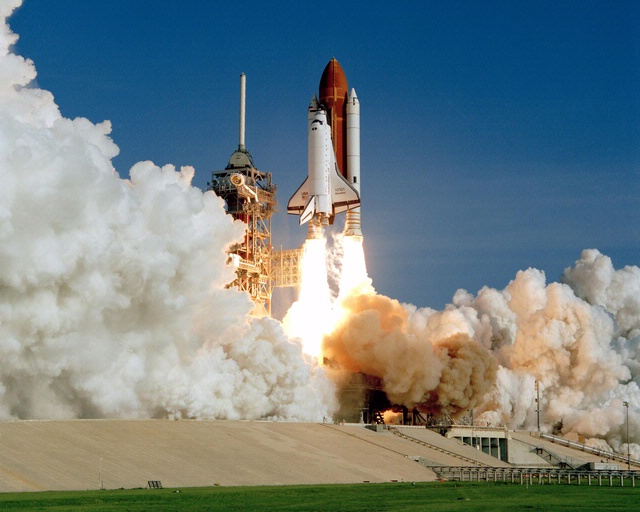
\includegraphics[scale=0.35]{gambar/roketluarangkasa.jpg}

%   % Ubah dengan keterangan gambar yang diinginkan
%   \caption{Peluncuran roket luar angkasa \emph{Discovery} \citep{roketluarangkasa}.}
%   \label{fig:roketluarangkasa}
% \end{figure}

% Roket luar angkasa merupakan \lipsum[1]

% \emph{Discovery}, Gambar \ref{fig:roketluarangkasa}, merupakan \lipsum[2]

% Per Teori Penunjang dibuat section baru

\section{\textit{Deep Learning}}
\label{sec:deeplearning}
\textit{Deep learning} (DL) merupakan cabang dari \textit{machine learning} yang didasarkan pada \textit{artificial neural network}.DL memungkinkan model komputasi dari beberapa lapisan pemrosesan untuk mempelajari dan mewakili data dengan berbagai tingkat abstraksi. \textit{Deep learning} merupakan metode yang memiliki implementasi sangat banyak mencakup \textit{Neural Networks, hierarchical probabilistic models, unsupervised} dan \textit{supervised learning} \citep*{voulodimos2018deep}. \textit{Deep Learning} dirancang untuk dapat terus mengolah data dan menganalisa data tersebut seperti dalam mengambil keputusan. Adapun dalam \textit{Deep Learning, training} suatu data dipengaruhi oleh banyaknya jumlah layer dan jumlah neuron. Artinya, semakin banyak layer atau neuron yang digunakan maka akan semakin lama proses yang dilakukan, hal ini disebabkan oleh tingkat kompleksitas yang semakin besar juga. \par

% not good
\section{Convolutional Neural Network (CNN)}
\label{sec:convolutionalneuralnetwork}
CNN merupakan algoritma \textit{deep learning}yang mampu mengambil masukan berupa gambar, menetapkan prioritas untuk berbagai aspek/objek dalam gambar dan mampu membedakan satu sama lain. Tahapan \textit{pre-processing} yang dibutuhkan CNN lebih sedikit jika dibandingkan dengan algoritma klasifikasi lainnya \citep*{towardsDS}. \textit{Convolutional Neural Network (CNN)} itu sendiri juga merupakan pengembangan dari \textit{Multilayer Percepton (MLP)} yang didesain untuk mengolah data dua dimensi. CNN termasuk dalam jenis \textit{Deep Neural Network} karena kedalaman jaringan yang tinggidan banyak diaplikasikan pada data citra \citep*{putra2016klasifikasi}.\par
Secara sederhana, CNN memiliki beberapa jenis \textit{neural layers} yang masing-masing memiliki peranannya masing-masing \citep*{voulodimos2018deep}. Adapun secara sederhana CNN terdiri dari 3 jenis utama \textit{neural layers} yaitu: \par
\begin{enumerate}[nolistsep]
    \item \textit{Convolutional Layers}
    \item \textit{Pooling Layers}
    \item \textit{Fully Connected Layers}
\end{enumerate}
\indent Secara umum, cara kerja CNN hampir serupa pada MLP, hanya saja dalam CNN setiap neuron dipresentasikan dalam bentuk dua dimensi. Adapun cara kerja dari suatu MLP sederhana yaitu MLP semula memiliki sejumlah \textit{layer} dengan masing-masing layer memiliki sejumlah \textit{neuron}. MLP menerima masukan data dalam bentuk satu dimensi, kemudian mempropagasikan data tersebut pada jaringan sehingga didapat hasil keluaran. Setiap hubungan antar \textit{neuron} pada dua \textit{layer} yang bersebelahan memiliki parameter bobot satu dimensi yang menentukan kualitas mode. Disetiap data input pada layer dilakukan operasi linear dengan nilai bobot yang ada, kemudian hasil komputasi akan ditransformasi menggunakan operasi non linear yang disebut sebagai fungsi aktivasi. \par


\section{Confusion Matrix}
\label{sec:confusionmatrix}

\section{Mean Average Precision (mAP)}
\label{sec:meanaverageprecision}

\section{Object Detection}
\label{sec:objectdetection}
\textit{Object Detection} adalah sebuah proses untuk mendeteksi suatu instance objek semantik dari kelas tertentu (seperti bentuk, huruf, pesawat, angka, dan lain lain) dalam sebuah gambar atau video. Pendekatan umum dari  \textit{frameworks} deteksi objek mencakupi pembuatan set besar yang diklasifikasikan secara sekuel menggunakan fitur CNN \citep*{voulodimos2018deep}. \par

% keknya gaperlu ??
% \section{Word Segmentation}
% \label{sec:wordsegmentation}
% Pengenalan tulisan tangan merupakan Teknik untuk menginterpretasikan tulisan tangan kedalam bentuk digital. Proses pengenalan tulisan tangan dapat diperoleh dengan 2 cara yaitu dengan mengonversi otomatis karakter pada saat ditulis pada layar sentuh dengan pena digital dan cara lain yaitu dengan melakukan pengambilan gambar serta pemrosesan gambar pada suatu teks yang ingin dikenali [8]. Pada proses segmentasi huruf, mulanya dokumen gambar disegmentasi kedalam baris-baris teks. Kemudian, algoritma segmentasi huruf diterapkan pada satu baris teks tersebut. Pada satu baris teks tersebut, secara umum proses segmentasi huruf konvensional menjalankan algoritma yang terdiri dari 2 tahapan yaitu: ekstraksi kandidat huruf berdasarkan pemisah huruf dan dilanjut dengan klasifikasi kandidat huruf \citep*{ryu2015word}.

\section{You Only Look Once (YOLO)}
\label{sec:yolo}
YOLO merupakan salah satu arsitektur dari CNN yang dioptimasi untuk mendeteksi objek pada gambar. Arsitektur YOLO sangat cepat apabila dibandingkan dengan arsitektur pengenalan objek lainnya . YOLO melakukan proses pengenalan objek berbasis CNN dalam sebuah kotak yang disebut \textit{anchor} yang dipusatkan pada 13x13 \textit{grid cell} dalam sebuah gambar. Artinya, ukuran gambar diubah (dikurangi) menjadi 416x416 terlepas dari ukuran asli dari gambar yang ingin di proses \textit{train or detect}. Artinya, jika terdapat perbedaan besar dalam rasio gambar yang diproses \textit{train}, maka akan terjadi distorsi serius pada objek ketika dilakukan proses penyesuaian ukuran\citep*{jeong2018image}. \par

% Kemudian menjadi persamaan seperti pada persamaan \ref{eq:hukumpertamanewton}.

% % Contoh pembuatan persamaan
% \begin{equation}
%   \label{eq:hukumpertamanewton}
%   \sum \mathbf{F} = 0\; \Leftrightarrow\; \frac{\mathrm{d} \mathbf{v} }{\mathrm{d}t} = 0.
% \end{equation}

  \cleardoublepage

  % Bab 3 desain dan implementasi
  % not fixed

\chapter{METODOLOGI}
\label{chap:metodologi}

% Ubah bagian-bagian berikut dengan isi dari desain dan implementasi

Penelitian ini dilaksanakan sesuai dengan desain sistem juga dengan implementasinya. Desain sistem merupakan konsep dari pembuatan dan perancangan infrastruktur dan kemudian diwujudkan dalam bentuk blok-blok alur yang harus dikerjakan. Pada bagian implementasi merupakan pelaksanaan teknis untuk setiap blok pada desain sistem.

\begin{figure}[H]
    \centering
    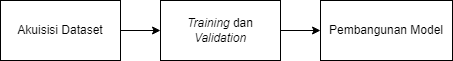
\includegraphics[scale=0.85]{gambar/metodologi_umum.png}
    \caption{Desain Sistem Keseluruhan}
    \label{fig:desainsistem}
\end{figure}

\section{Peralatan}
\label{sec:peralatan}
Peralatan yang digunakan pada penelitian ini yaitu Laptop. Laptop, digunakan pada keseluruhan implementasi metodologi ini. Adapun spesifikasi laptop yang digunakan pada penelitian ini adalah laptop dengan spesifikasi seperti pada tabel \ref{tb:spesifikasilaptop}.\par

\begin{table}[H]
    \begin{center}
        \begin{tabular}{|l|l|}
        \hline
        \textit{\textbf{Processor}}        & \begin{tabular}[c]{@{}l@{}}Intel Core i5-8300H \\ CPU @ 2.3 GHz (8 CPUs)\end{tabular} \\ \hline
        \textit{\textbf{Storage}}          & \begin{tabular}[c]{@{}l@{}}HDD 1 TB Storage\\ SSD 256 GB Storage\end{tabular}         \\ \hline
        \textit{\textbf{RAM}}              & \begin{tabular}[c]{@{}l@{}}16 GB SODIMM DDR4 \\ 2667 MHz Dual Channel\end{tabular}    \\ \hline
        \textit{\textbf{Graphic Card}}     & \begin{tabular}[c]{@{}l@{}}NVIDIA GeForce GTX 1050 Ti \\ 4 GB GDDR5\end{tabular}      \\ \hline
        \textit{\textbf{Operating System}} & \begin{tabular}[c]{@{}l@{}}Windows 10 Home \\ Single Language 64-bit\end{tabular}     \\ \hline
    \end{tabular}
    \caption{Spesifikasi Laptop yang Digunakan}
    \label{tb:spesifikasilaptop}
    \end{center}
\end{table}

\section{Desain Sistem}
\label{sec:desainsistem}

Tugas akhir ini merupakan penelitian dalam bidang visi komputer yang bertujuan untuk mendeteksi huruf balok tulisan tangan pada media papan tulis menggunakan metode \textit{you only look once} (YOLO). Adapun secara umum alur desain sistem yaitu seperti pada gambar \ref*{fig:desainsistem}. Perancangan model menggunakan metode YOLO, lebih spesifik yaitu YOLOv5. \par

Berdasarkan gambar \ref*{fig:desainsistem}, langkah awal yang harus dilakukan yaitu proses akuisisi dataset, yaitu dengan mengumpulkan data tulisan tangan huruf balok pada media papan tulis dan setelahnya juga dilakukan pre-proses tertentu yang akan dijelaskan pada sub akuisisi data. Proses selanjutnya yaitu dengan melakukan konfigurasi-konfigurasi pada model sebelum dilakukan training, dan ketika sudah dilakukan proses training maka hasil model yang telah dibuat tersebut dievaluasi dengan confusion matrix. \par

% Per blok diagram dijelaskan dan dibuatkan section masing-masing

\section{Akuisisi Dataset}
\label{sec:akuisisidataset}

Dalam pelaksanaan proses akuisisi dataset, terdapat beberapa bagian proses yang harus dilakukan yang dapat dilihat pada blok diagram berikut.

\begin{figure}[ht]
    \centering
    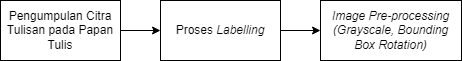
\includegraphics[scale=0.85]{gambar/metodologi_akuisisi_data.png}
    \caption{Alur Akuisisi Dataset}
    \label{fig:alurakuisisidataset}
\end{figure}

\subsection{Pengumpulan Citra Tulisan pada Papan Tulis}
\label{subsec:pengumpulancitra}

Proses pengumpulan citra huruf balok tulisan tangan pada papan tulis dimulai dengan menentukan jumlah kelas dataset yang akan digunakan. Pada huruf alfabet, terdapat 26 huruf dari A sampai Z yang artinya pada proses akuisisi dataset ini nantinya akan terdapat 26 kelas yang mewakili masing-masing huruf tersebut. Setelah jumlah kelas ditentukan, proses selanjutnya yaitu membuat huruf balok tulisan tangan pada media papan tulis kemudian mengambil gambar dari huruf balok tulisan tangan tersebut. Proses tersebut diulang sebanyak beberapa kali pada tiap kelas yang sama dan diulang kembali sesuai jumlah kelas yang tersedia. \par

\subsection{Proses Pelabelan Dataset}
\label{subsec:proseslabelling}

Proses pelabelan yaitu merupakan proses pemberian label dengan memberikan \textit{bounding box} pada objek dan nama kelas pada objek tersebut. Tujuan dari proses pelabelan ini yaitu untuk mendapatkan \textit{ground-truth bounding box}. Proses pelabelan dilakukan dengan menggunakan bantuan \textit{tool} yaitu Roboflow. Sebelum proses pelabelan dilakukan, citra yang telah dikumpulkan sebelumnya diupload pada \textit{workspace} Roboflow. Setelah diberikan \textit{bounding box}, citra yang telah diberikan label selanjutnya dibagi menjadi \textit{training sets} dan \textit{testing sets}. \par
% Adapun pembagian \textit{training testing sets} menggunakan komposisi 80\% \textit{training sets} dan 20\% \textit{testing sets}. \par

\subsection{\textit{Image Pre-Processing}}
\label{subsec:imagepreprocess}

Pada tahapan \textit{image pre-processing} ini dilakukan 3 jenis pre-proses yaitu \textit{resize, grayscalling}, dan \textit{bounding box rotation}. Pada proses \textit{resize}, citra yang telah diambil ukurannya diperkecil (diregangkan) menjadi ukuran 416x416, hal ini bertujuan untuk memperkecil ukuran file serta mempercepat proses \textit{training} mengingat jumlah data dan jumlah kelas yang banyak. \par

Pada proses \textit{grayscalling}, gambar dibuat menjadi warna abu dengan tujuan untuk memperkecil variasi warna spidol pada media papan tulis sehingga model yang dibuat berfokus hanya pada pola tulisan tangan pada papan tulis saja dan tidak terfokus ke warna yang digunakan untuk menulis pada papan tulisnya. \par

Terakhir, dilakukan proses \textit{bounding box rotation} seperti pada gambar \ref*{fig:bbrotation}, yaitu melakukan rotasi pada skala \textit{bounding box}, tujuannya untuk menambah variasi sehingga model yang tercipta lebih akurat ketika pengambilan citra tidak diambil tepat didepan objek. Adapun konfigurasi dari \textit{bounding box rotation} yaitu antara -15\textdegree\space dan +15\textdegree. \par
% perlu g y tabel konfigurasi preproses yang digunakan

\section{Training}
\label{sec:trainingdata}

\textit{Training data} dilakukan setelah proses pengumpulan citra, proses pelabelan, dan pre-proses gambar selesai dilaksanakan. Dalam proses \textit{training}, dibutuhkan konfigurasi \textit{hyperparameter} tertentu seperti jumlah epochs, \textit{batch size}, dan jenis \textit{pretrained weight} yang akan digunakan. Pada tugas akhir ini, versi YOLO yang digunakan yaitu YOLOv5. \par

Sebelum proses \textit{training} dilakukan, perlu ditentukan jenis \textit{pretrained weights} yang akan digunakan. Pada YOLOv5, terdapat beberapa jenis \textit{pretrained weights} yang tersedia yaitu YOLOv5n, YOLOv5s, YOLOv5m, YOLOv5l, dan YOLOv5x. Pada tugas akhir ini, \textit{pretrained weight} yang digunakan yaitu YOLOv5s. \par
% Adapun konfigurasi layer YOLOv5 secara lebih lengkap telah dibahas pada tinjauan pustaka ttg yolov5 

Setelah menentukan jenis \textit{pretrained weight} yang akan digunakan, selanjutnya yaitu menentukan konfigurasi \textit{hyperparameter} untuk data yang akan di-\textit{train}. Konfigurasi \textit{hyperparameter} yang dilakukan yaitu pengaturan epochs, \textit{batch size,} dan \textit{image size}. Adapun penjelasan dari masing-masing pengaturan yaitu: \par
\begin{enumerate}[nolistsep]
    \item \textbf{Epochs}. Epochs adalah \textit{hyperparameter} yang berfungsi untuk menentukan jumlah pengulangan atau berapa kali suatu algoritma \textit{learning} akan melakukan proses \textit{learning} suatu \textit{dataset training}. Secara sederhana, semakin besar jumlah epochs maka model yang dihasilkan memiliki tingkat akurasi yang lebih tinggi namun waktu yang dibutuhkan untuk melakukan \textit{learning} akan semakin lambat. Pada tugas akhir ini, epochs yang digunakan yaitu 30.
    \item \textit{\textbf{Batch-size}}. \textit{Batch-size} adalah \textit{hyperparameter} yang berfungsi untuk mengontrol jumlah sampel training untuk dikerjakan sebelum parameter internal model diperbarui. Pada tugas akhir ini, \textit{batch-size} yang digunakan yaitu 16.
    \item \textit{\textbf{Image Size}}. \textit{Image size} adalah ukuran gambar yang diterapkan pada \textit{dataset}. Pada tugas akhir ini, \textit{dataset} menggunakan \textit{image size} berukuran 416x416.
\end{enumerate}
% tambahkan tabel spesifikasi model yg digunakan

\section{Pembuatan Model}
\label{sec:pembuatanmodel}

Pada tahapan pembuatan model, setelah dilakukan proses \textit{training,} hasil tersebut akan tersimpan pada direktori 'runs/train/..'. Pada direktori tersebut didapatkan \textit{checkpoint} hasil model beserta dengan grafik atau detil data hasil pada tiap proses pengulangan. \par
% tampilkan gambar result.csv
% tampilkan hasil deteksi
Pada tahapan selanjutnya, ketika hasil model dirasa telah cukup bagus baik itu dari segi data angka performa maupun dari hasil proses deteksi, selanjutnya yaitu pembuatan algoritma konversi gambar menjadi teks. Proses penyusunan teks dimulai dari menentukan koordinat seluruh \textit{bounding box} yang tersedia. Setelah koordinat \textit{bounding box} didapat, seluruh \textit{bounding box} yang terbaca dikelompokan berdasarkan kedekatan antara \textit{bounding box} pertama dengan \textit{bounding box} selanjutnya, jika jarak antaranya memenuhi \textit{threshold} tertentu maka akan dikelompokan menjadi 1, dan jika tidak memenuhi maka akan diletakan pada kelompok berikutnya. Adapun prioritas pengelompokan diatur berdasarkan koordinat Y dahulu lalu dilanjutkan dengan koordinat X, hal ini bertujuan agar teks yang ditampilkan berurutan dari baris atas lalu bergerak kearah X+, dan dilanjut pada baris kedua dan seterusnya. Alur dari pembentukan algoritma konversi gambar menjadi teks dapat dilihat pada gambar berikut. \par
% tampilkan flowchart pembuatan  
% alur pembuatan model: start -> input gambar -> deteksi bounding box -> mencari xy bounding box -> pengelompokan berdasarkan y bounding box -> pengelompokan berdasarkan x bounding box -> konversi kelas menjadi bentuk string -> menampilkan label -> selesai

  \cleardoublepage

  % Bab 4 pengujian dan analisis
  \chapter{HASIL DAN PEMBAHASAN}
\label{chap:hasilpembahasan}

% Ubah bagian-bagian berikut dengan isi dari hasil dan pembahasan

Pada bab ini dipaparkan hasil dan analisa dari pelaksanaan tiap tahapan pada metodologi, serta dipaparkan mengenai skenario pengujian dan evaluasi pengujiannya. Pengujian dilakukan guna mengetahui tingkat kesalahan dan menarik kesimpulan dari metodologi serta analisis yang telah dibuat. Tahapan skenario pengujian meliputi hal berikut, yaitu: \par

\begin{enumerate}[nolistsep]
  \item Pengujian menggunakan \textit{pretrained weight} model yang bervariasi.
  \item Pengujian menggunakan \textit{input} citra tulisan dari responden berbeda.
  \item Pengujian menggunakan \textit{input} citra dengan jarak pengambilan citra bervariasi.
  \item Pengujian menggunakan \textit{input} citra dengan pencahayaan pengambilan citra bervariasi.
\end{enumerate}

Dengan hasil metodologi serta pelaksanaan skenario-skenario pengujian yang akan dipaparkan pada bab 4 ini, diharapkan mendapatkan hasil dan analisa sehingga dapat ditarik kesimpulan dari pelaksanaan tugas akhir ini. \par

\section{Hasil Metodologi}
\label{sec:hasilmetodologi}

Pada metodologi terdapat blok-blok diagram dan telah dilakukan pelaksanaan tugas akhir sesuai dengan blok diagram tersebut. Adapun hasil dari tiap tahapan yang dilakukan pada blok diagram tersebut secara rinci akan dijelaskan pada sub berikut. \par
% ini dijelaskan sesuai dengan metodologi yang telah dibuat sebelumnya. \par

\subsection{Hasil Akuisisi Dataset}
\label{subsec:Hasilakuisisidataset}

Pada tahapan akuisisi dataset, secara umum pelaksanaannya terbagi dalam 3 tahapan yaitu pengumpulan citra tulisan tangan pada papan tulis, proses pelabelan, dan proses \textit{image pre-processing.} Pada tahapan akuisisi dataset, secara umum didapatkan hasil jumlah dataset seperti pada Tabel \ref*{tb:hasilakuisisidata} serta proses \textit{pre-process} secara singkat seperti pada Tabel \ref*{tb:checklistpreprocess}.

% //FIXME: perbarui detail preproses dataset
\begin{center}
  \begin{longtable}[c]{|l|l|}
    \hline
    \multicolumn{1}{|c|}{\textbf{Jenis \textit{Pre-Process}}} & \multicolumn{1}{c|}{\textbf{Keterangan}} \\ \hline
    \endfirsthead
    \endhead
    \textit{Auto Orient}                             & Diterapkan                                               \\ \hline
    \textit{Resize}                                  & \textit{Stretch to} 416x416                              \\ \hline
    \textit{Grayscale}                               & Diterapkan                                               \\ \hline
    \textit{Contrast}                                & \textit{Contrast Stretching}                             \\ \hline
    \textit{Filter Null}                             & Diterapkan                                               \\ \hline
    \textit{Blur}                                    & \textit{Random up to 8px}                                \\ \hline
    \textit{Noise}                                   & \textit{Random up to 2\% pixels}                         \\ \hline
    \textit{Bounding Box Rotation}                   & \textit{Random between -5\textdegree and +5\textdegree}  \\ \hline
    \caption{Tahapan Pre-Process yang Dilakukan}
    \label{tb:checklistpreprocess}\\
  \end{longtable}
\end{center}

% //FIXME: perbarui detail kelas dataset
\begin{center}
  \begin{longtable}[c]{|c|c|c|c|c|}
    \hline
    \textbf{Kelas} & \textbf{Jumlah Citra} & \multicolumn{1}{l|}{\textbf{Jumlah Anotasi}} & \multicolumn{1}{l|}{\textit{\textbf{Train Set}}} & \multicolumn{1}{l|}{\textit{\textbf{Validation Set}}} \\ \hline
    \endfirsthead
    \endhead
    *              & 36           & 540         & 29         & 7         \\ \hline
    =              & 50           & 750         & 45         & 5         \\ \hline
    0              & 50           & 750         & 45         & 5         \\ \hline
    1              & 50           & 750         & 45         & 5         \\ \hline
    2              & 50           & 750         & 45         & 5         \\ \hline
    3              & 50           & 750         & 45         & 5         \\ \hline
    4              & 50           & 750         & 45         & 5         \\ \hline
    5              & 50           & 750         & 45         & 5         \\ \hline
    6              & 50           & 750         & 45         & 5         \\ \hline
    7              & 50           & 750         & 45         & 5         \\ \hline
    8              & 50           & 750         & 45         & 5         \\ \hline
    9              & 50           & 750         & 45         & 5         \\ \hline
    A              & 50           & 750         & 45         & 5         \\ \hline
    B              & 50           & 750         & 45         & 5         \\ \hline
    D              & 50           & 750         & 45         & 5         \\ \hline
    E              & 50           & 750         & 45         & 5         \\ \hline
    G              & 50           & 750         & 45         & 5         \\ \hline
    I              & 50           & 750         & 45         & 5         \\ \hline
    J              & 50           & 750         & 45         & 5         \\ \hline
    K              & 50           & 750         & 45         & 5         \\ \hline
    L              & 50           & 750         & 45         & 5         \\ \hline
    M              & 50           & 750         & 45         & 5         \\ \hline
    N              & 50           & 750         & 45         & 5         \\ \hline
    P              & 50           & 750         & 45         & 5         \\ \hline
    R              & 50           & 750         & 45         & 5         \\ \hline
    S              & 50           & 750         & 45         & 5         \\ \hline
    T              & 50           & 750         & 45         & 5         \\ \hline
    U              & 50           & 750         & 45         & 5         \\ \hline
    V              & 50           & 750         & 45         & 5         \\ \hline
    \caption{Hasil Akuisisi Data}
    \label{tb:hasilakuisisidata}\\
  \end{longtable}
\end{center}

Secara spesifik, hasil dari tiap proses yang ada pada tahapan akuisisi dataset akan dijelaskan pada poin-poin berikut. \par

\subsubsection{Hasil Pengumpulan Citra Tulisan Tangan pada Papan Tulis}
\label{subsubsec:hasilpengumpulancitra}

Proses pengumpulan citra tulisan tangan papan tulis dilakukan dengan menuliskan sejumlah huruf, angka, dan simbol pada media papan tulis kemudian dilakukan proses pengambilan citra. Proses tersebut dilakukan secara berulang sampai jumlah tertentu untuk suatu kelas yang sama dan diulang kembali dengan kelas berbeda sampai seluruh jumlah kelas terpenuhi. Seluruh tulisan tangan pada papan tulis ditulis oleh 1 orang yang sama. Pada saat proses pengambilan citra, citra diambil dengan perangkat \textit{smartphone} yang detail spesifikasinya dapat dilihat pada Tabel \ref*{tb:spesifikasismartphone}. Dalam proses pengambilan citra, terdapat beberapa teknik berbeda dalam pengambilan citra, yaitu: pengambilan citra dengan intensitas cahaya berbeda (diatur menggunakan kamera penulis) dan pengambilan citra dengan sudut pengambilan citra yang berbeda. Hal tersebut dilakukan agar tiap kelas yang ada memiliki variasi sehingga ketika model diterapkan secara langsung dapat mendeteksi dari berbagai kondisi. Contoh hasil dari pengambilan citra dengan variasi intensitas cahaya dapat dilihat pada Gambar \ref{fig:intensitascitrabervariasi} dan contoh hasil dari pengambilan citra dengan variasi sudut pengambilan gambar dapat dilihat pada Gambar \ref*{fig:pengambilancitrabervariasi}.  \par

\begin{figure}[H]
  \begin{subfigure}{.5\textwidth}
    \centering
    \captionsetup{width=.8\linewidth}
    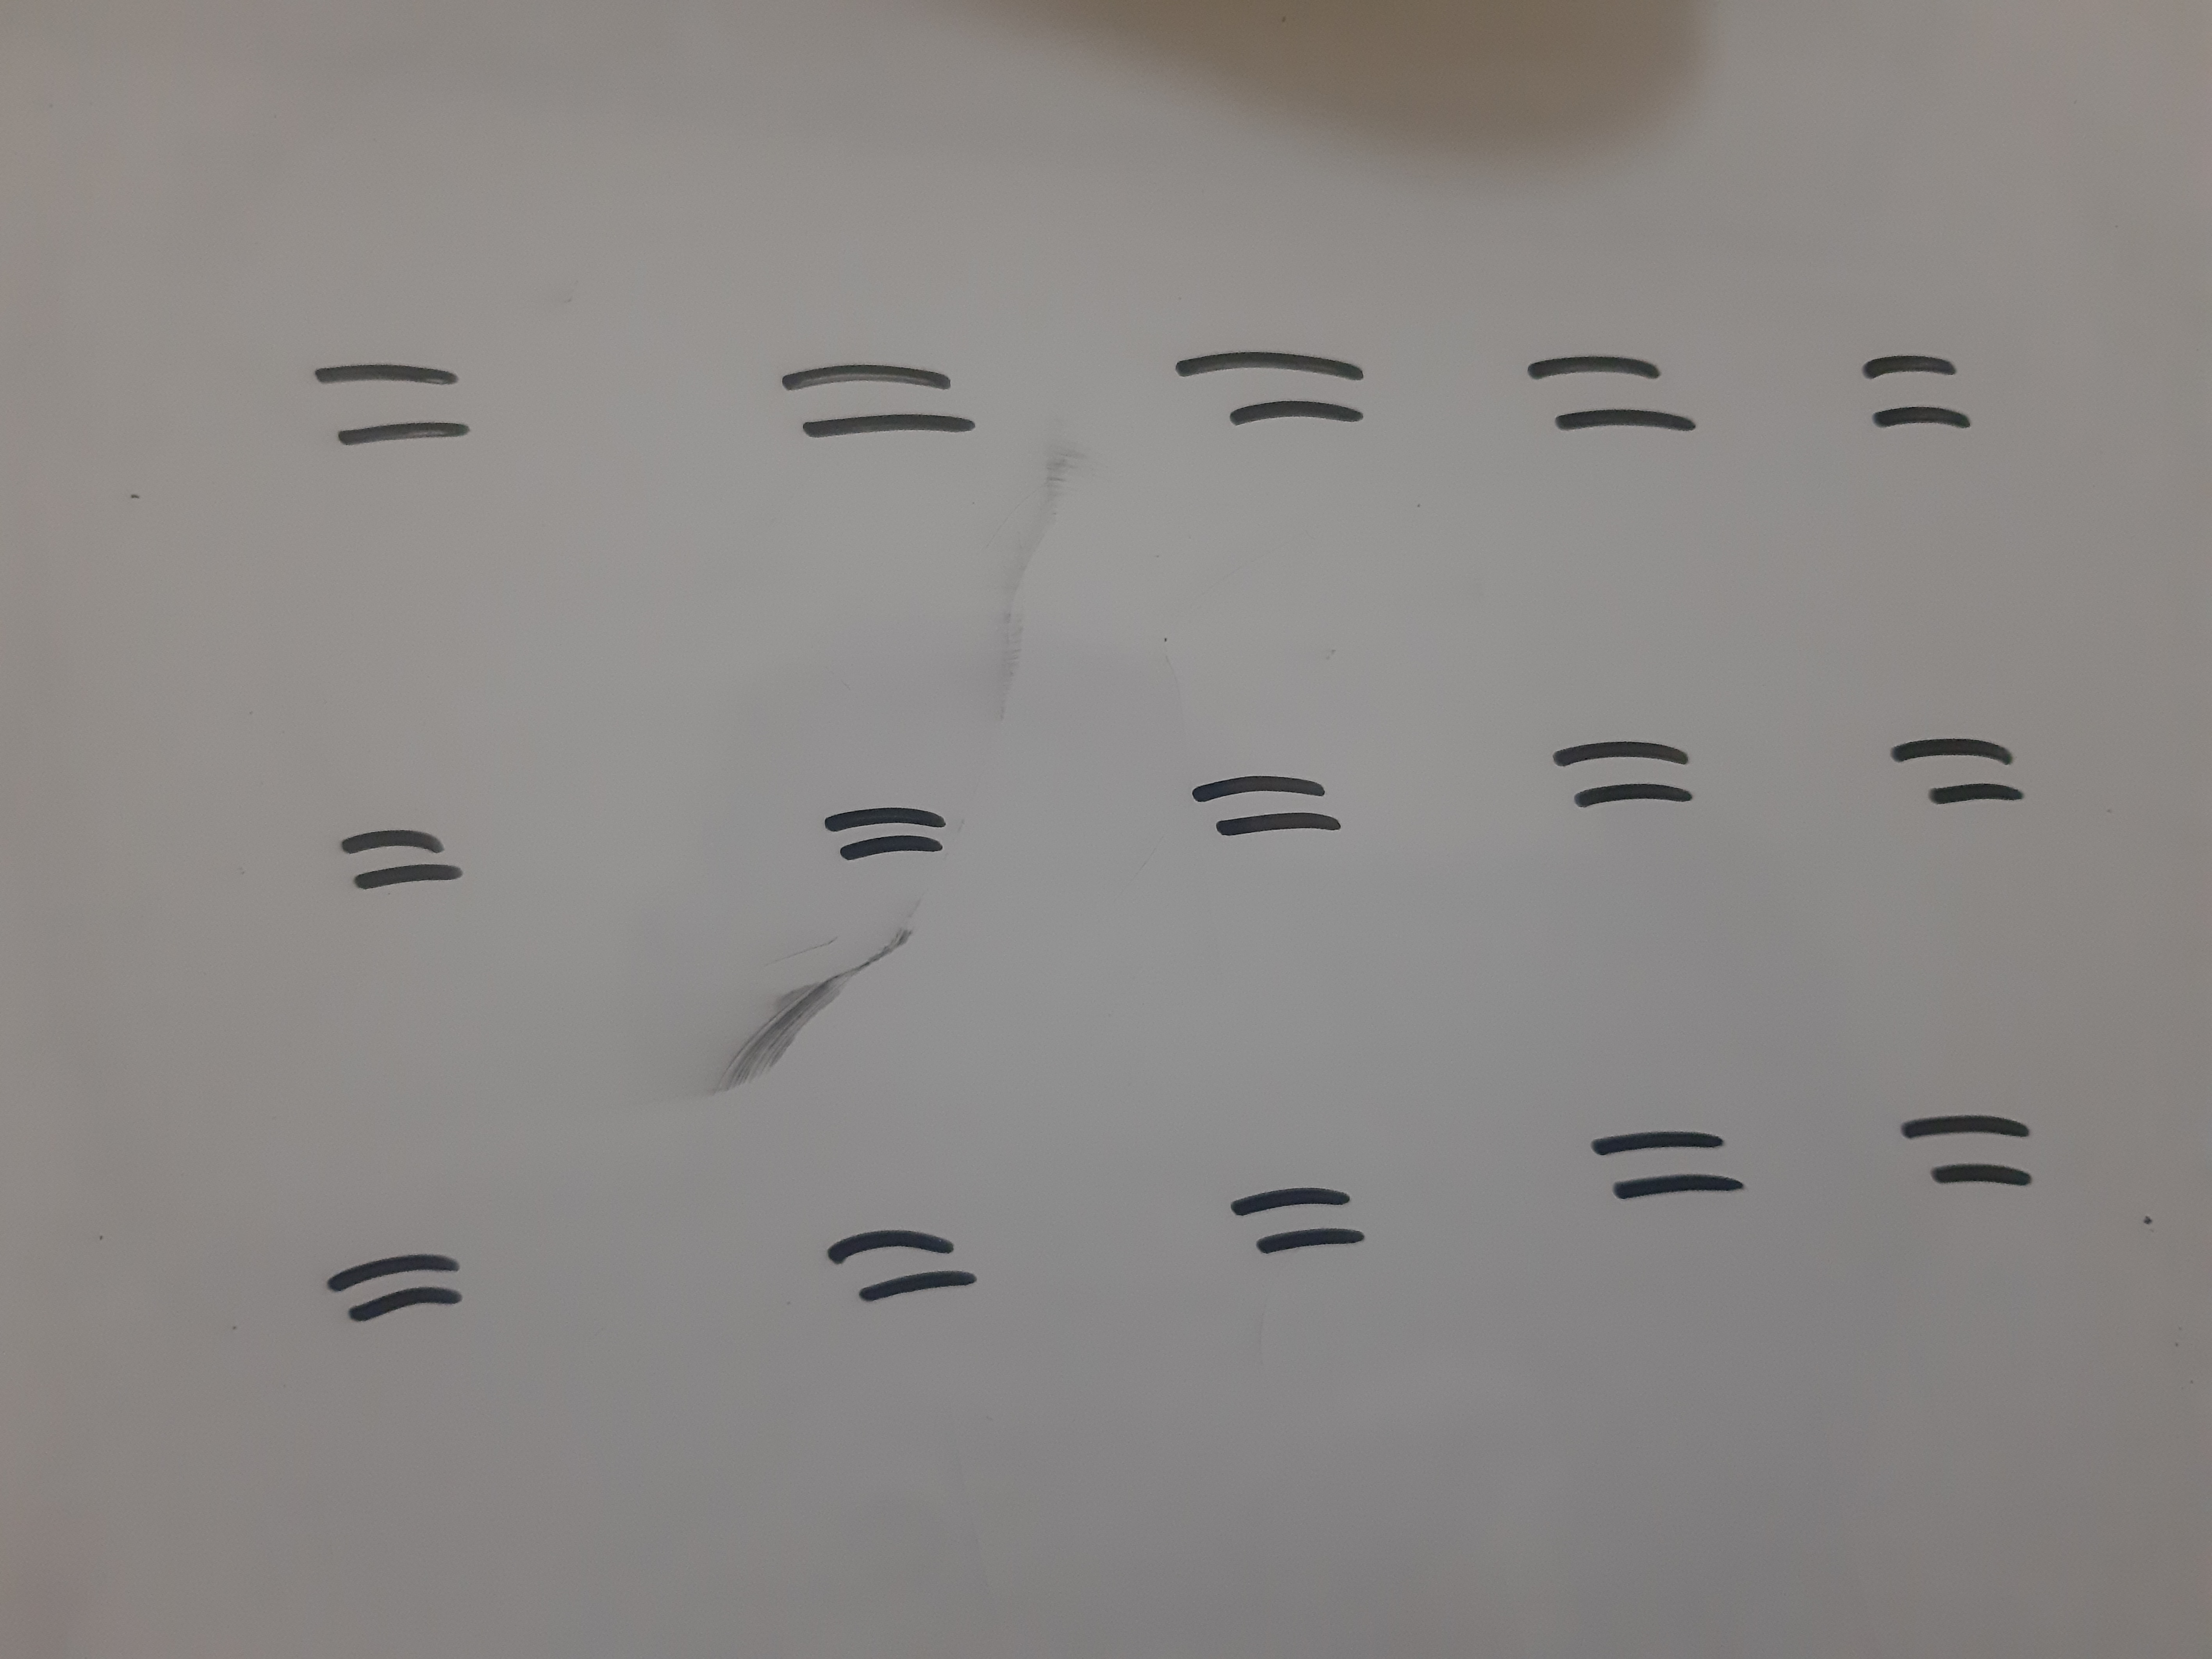
\includegraphics[width=.85\linewidth]{gambar/pengambilan_citra_terang.jpg}
    \caption{Pengambilan Citra dengan Kondisi Normal}
    \label{fig:citraterang}
  \end{subfigure}%
  \begin{subfigure}{.5\textwidth}
    \centering
    \captionsetup{width=.8\linewidth}
    \includegraphics[width=.85\linewidth]{gambar/pengambilan_citra_gelap.jpg}
    \caption{Pengambilan Citra dengan Kondisi \textit{Apperture} Kisaran -1 \textit{Steps.}}
    \label{fig:citragelap}
  \end{subfigure}
  \caption{Pengambilan Citra dengan Variasi Intensitas Cahaya}
  \label{fig:intensitascitrabervariasi}
\end{figure}

\begin{figure}[H]
  \begin{subfigure}{.5\textwidth}
    \centering
    \captionsetup{width=.8\linewidth}
    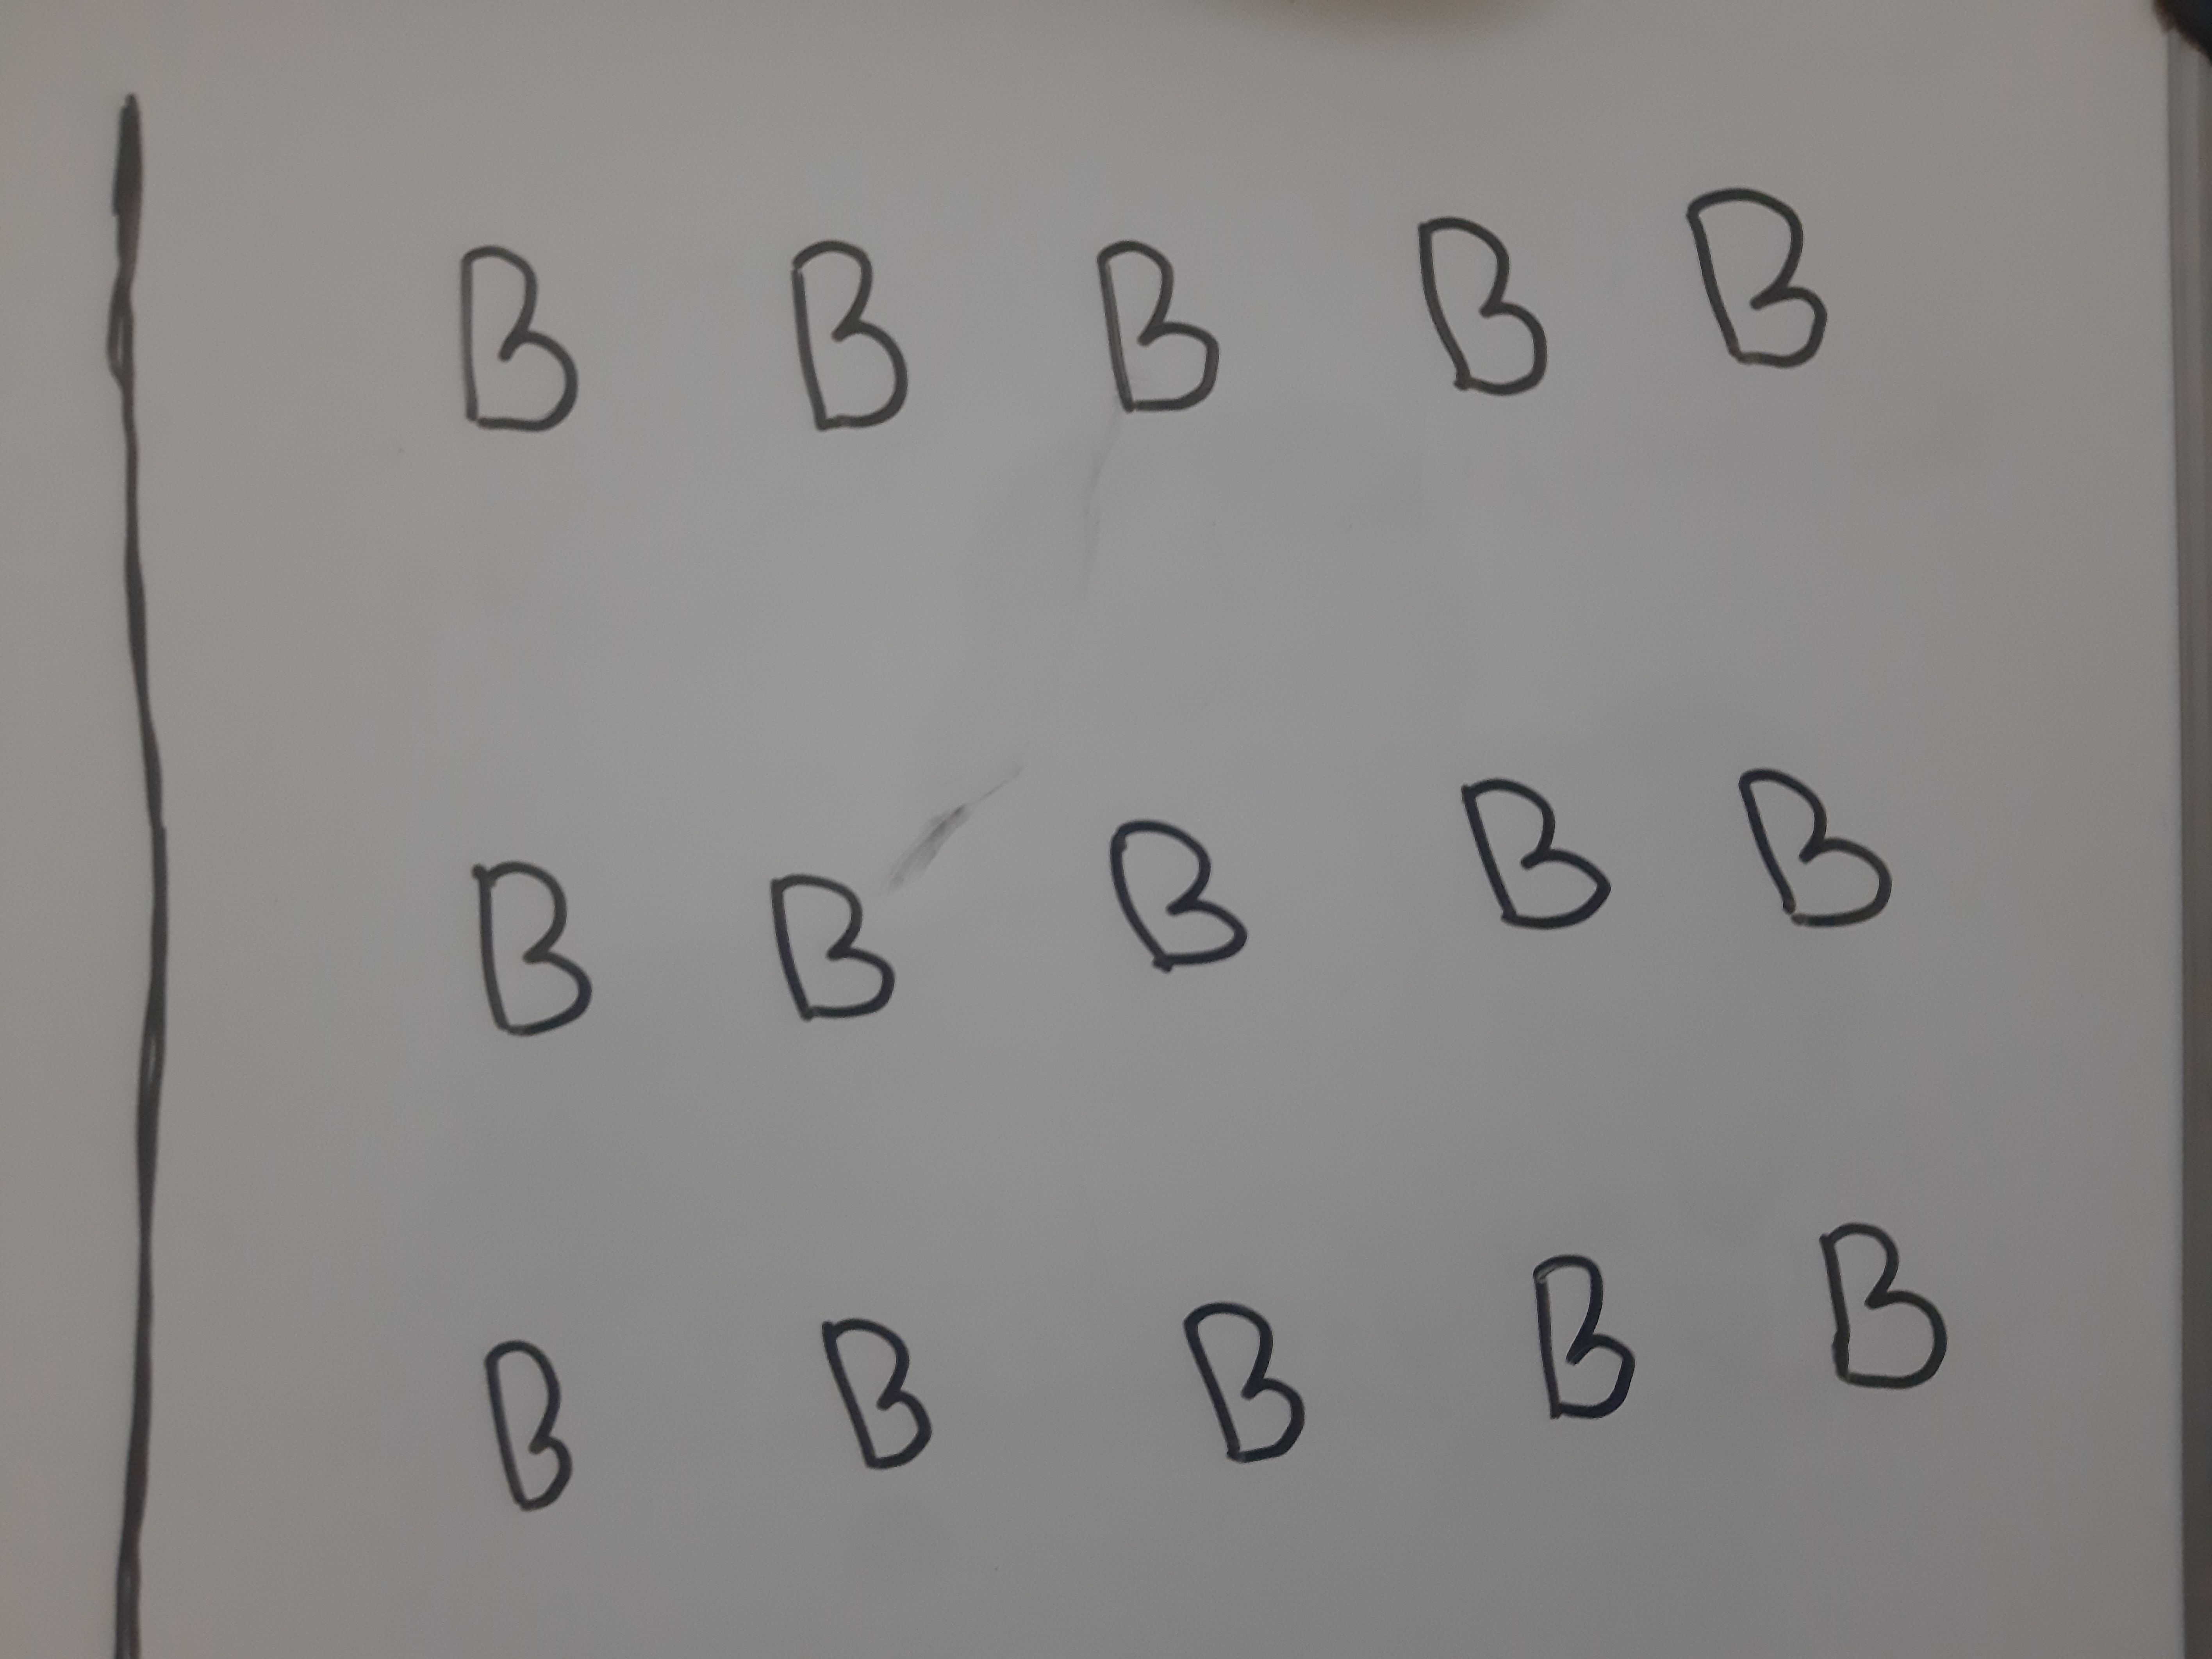
\includegraphics[width=.85\linewidth]{gambar/pengambilan_citra_depan.jpg}
    \caption{Pengambilan Citra dari Depan}
    \label{fig:citradepan}
  \end{subfigure}%
  \begin{subfigure}{.5\textwidth}
    \centering
    \captionsetup{width=.8\linewidth}
    \includegraphics[width=.85\linewidth]{gambar/pengambilan_citra_samping.jpg}
    \caption{Pengambilan Citra dari Samping}
    \label{fig:citrasamping}
  \end{subfigure}
  \caption{Pengambilan Citra dengan Variasi Sudut Pengambilan Gambar}
  \label{fig:pengambilancitrabervariasi}
\end{figure}

Secara spesifik, total persebaran citra pada masing-masing kelas dapat dilihat pada Tabel \ref{tb:citrapadatiapkelas} berikut. \par

% //FIXME: perbarui tabel
\begin{center}
  \begin{longtable}{|c|c|c|c|}
    \hline
    \textbf{Kelas} & \textbf{Jumlah Gambar} & \textbf{\textit{Train Sets}} & \textbf{\textit{Test Sets}} \\ \hline
      *                                    & 36                     & 29                  & 7                  \\ \hline
      =                                    & 50                     & 45                  & 5                  \\ \hline
      0                                    & 50                     & 45                  & 5                  \\ \hline
      1                                    & 50                     & 45                  & 5                  \\ \hline
      2                                    & 50                     & 45                  & 5                  \\ \hline
      3                                    & 50                     & 45                  & 5                  \\ \hline
      4                                    & 50                     & 45                  & 5                  \\ \hline
      5                                    & 50                     & 45                  & 5                  \\ \hline
      6                                    & 50                     & 45                  & 5                  \\ \hline
      7                                    & 50                     & 45                  & 5                  \\ \hline
      8                                    & 50                     & 45                  & 5                  \\ \hline
      9                                    & 50                     & 45                  & 5                  \\ \hline
      A                                    & 36                     & 29                  & 7                  \\ \hline
      B                                    & 30                     & 27                  & 3                  \\ \hline
      D                                    & 36                     & 29                  & 7                  \\ \hline
      E                                    & 36                     & 29                  & 7                  \\ \hline
      G                                    & 36                     & 29                  & 7                  \\ \hline
      H                                    & 36                     & 29                  & 7                  \\ \hline
      I                                    & 36                     & 29                  & 7                  \\ \hline
      J                                    & 36                     & 29                  & 7                  \\ \hline
      K                                    & 36                     & 29                  & 7                  \\ \hline
      L                                    & 36                     & 29                  & 7                  \\ \hline
      M                                    & 20                     & 16                  & 4                  \\ \hline
      N                                    & 20                     & 16                  & 4                  \\ \hline
      P                                    & 36                     & 29                  & 7                  \\ \hline
      R                                    & 36                     & 29                  & 7                  \\ \hline
      S                                    & 36                     & 29                  & 7                  \\ \hline
      T                                    & 36                     & 29                  & 7                  \\ \hline
      U                                    & 36                     & 29                  & 7                  \\ \hline
      V                                    & 36                     & 29                  & 7                  \\ \hline
      W                                    & 36                     & 29                  & 7                  \\ \hline 
    \caption{Jumlah Citra Pada Tiap Kelas}
    \label{tb:citrapadatiapkelas}
  \end{longtable}
\end{center}
  
\subsubsection{Hasil Proses Pelabelan Dataset}
\label{subsubsec:hasilpelabelan}

Proses pelabelan dilakukan dengan memberikan \textit{bounding box} pada tiap-tiap citra yang telah dikumpulkan pada tahap sebelumnya. Pada proses \textit{bounding box,} tiap-tiap citra yang termasuk sebagai objek dari tiap kelas dianotasi sehingga seluruh bagian objeknya berada didalam anotasi dan diberi label sesuai dengan kelas objeknya. Anotasi pada proses pelabelan ini menggunakan anotasi berbentuk segiempat. Setelah proses pelabelan dilakukan maka \textit{output} yang dihasilkan pada tiap citra yang diolah yaitu sebuah file citra yang sudah di-\textit{pre-process} dan sebuah file txt berisi titik koordinat dari tiap objek yang ada pada sebuah citra tersebut. Adapun proses pelabelan dataset dapat dilihat pada Gambar \ref{fig:labellingroboflow}. 

\begin{figure}[H]
  \centering
  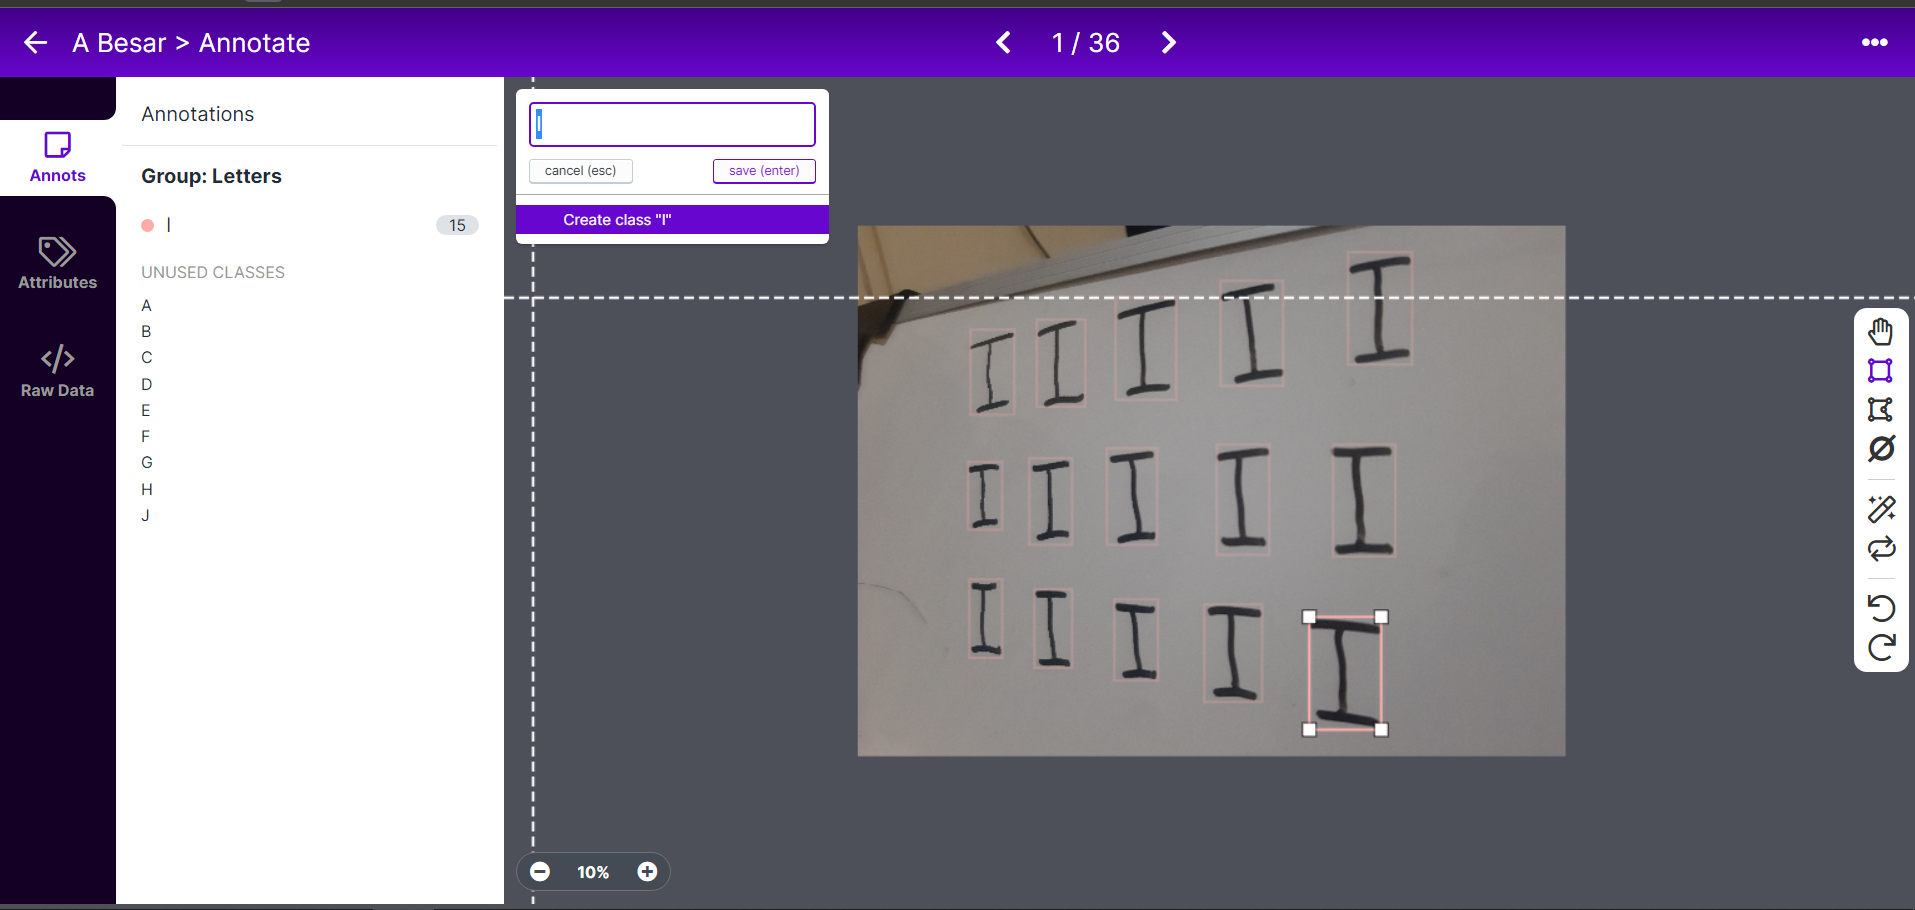
\includegraphics[scale=0.39]{gambar/labelling.png}
  \caption{Proses Pelabelan menggunakan Roboflow}
  \label{fig:labellingroboflow}
\end{figure}

Setelah dilakukan proses pelabelan, \textit{output} yang dihasilkan yaitu gambar yang memiliki \textit{bounding box}, dan apabila di-\textit{export} maka dataset hasil pelabelan terdiri dari 2 file yaitu file citra itu sendiri dan juga file txt yang berisi koordinat \textit{bounding box} yang ada pada suatu citra tersebut. Adapun total persebaran anotasi \textit{bounding box} pada masing-masing kelas dapat dilihat pada Tabel \ref{tb:anotasitiapkelas} berikut. 

% //FIXME: perbarui datanya
\begin{center}
  \begin{longtable}{|c|c|}
  \hline
  \textbf{Kelas} & \textbf{Jumlah Anotasi} \\ \hline
  A                                    & 540                     \\ \hline
  B                                    & 540                     \\ \hline
  C                                    & 540                     \\ \hline
  D                                    & 540                     \\ \hline
  E                                    & 900                     \\ \hline
  F                                    & 900                     \\ \hline
  G                                    & 540                     \\ \hline
  H                                    & 540                     \\ \hline
  I                                    & 540                     \\ \hline
  J                                    & 540                     \\ \hline
  K                                    & 540                     \\ \hline
  L                                    & 540                     \\ \hline
  M                                    & 900                     \\ \hline
  N                                    & 900                     \\ \hline
  O                                    & 540                     \\ \hline
  P                                    & 540                     \\ \hline
  Q                                    & 540                     \\ \hline
  R                                    & 540                     \\ \hline
  S                                    & 540                     \\ \hline
  T                                    & 540                     \\ \hline
  U                                    & 900                     \\ \hline
  V                                    & 900                     \\ \hline
  W                                    & 900                     \\ \hline
  X                                    & 540                     \\ \hline
  Y                                    & 540                     \\ \hline
  Z                                    & 540                     \\ \hline
  \caption{Jumlah Anotasi Pada Tiap Kelas}
  \label{tb:anotasitiapkelas}
  \end{longtable}
\end{center}
  

\subsubsection{Hasil \textit{Image Pre-Processing}}
\label{subsubsec:hasilpreprocess}

Pada tahap \textit{pre-process}, citra yang telah diberi label selanjutnya dilakukan \textit{pre-process} tertentu. Tahapan \textit{pre-process} bertujuan untuk mengurangi waktu \textit{training} dan meningkatkan performa. Secara ringkas, tahapan \textit{pre-process} yang dilakukan yaitu seperti pada Tabel \ref*{tb:checklistpreprocess}. Secara spesifik, pada tahapan \textit{pre-process} melakukan proses transformasi citra tertentu yaitu:
\begin{enumerate}[nolistsep]
% //TODO: pertimbangkan menggunakan noise pada preproses
  \item \textit{\textbf{Auto Orient.} Auto Orient} dilakukan untuk agar citra yang ditampilkan orientasinya sesuai dengan ketika diambil pada pengambilan awal.
  \item \textit{\textbf{Resize.} Resize} dilakukan untuk mengubah dimensi citra menjadi lebih kecil. Citra diubah dengan pengaturan \textit{stretch} sehingga tiap citra yang sebelumnya tidak memiliki dimensi ukuran 416x416 diregangkan ukurannya menjadi ukuran 416x416.
  \item \textit{\textbf{Grayscale.} \textnormal{Proses} Grayscale} bertujuan untuk memperkecil variasi warna gambar khususnya objek yang dibuat dengan spidol sehingga proses \textit{train} menjadi lebih cepat. Hasil dari proses \textit{grayscale} seperti pada Gambar \ref{fig:grayscallingdataset}.
    \begin{figure}[H]
      \centering
      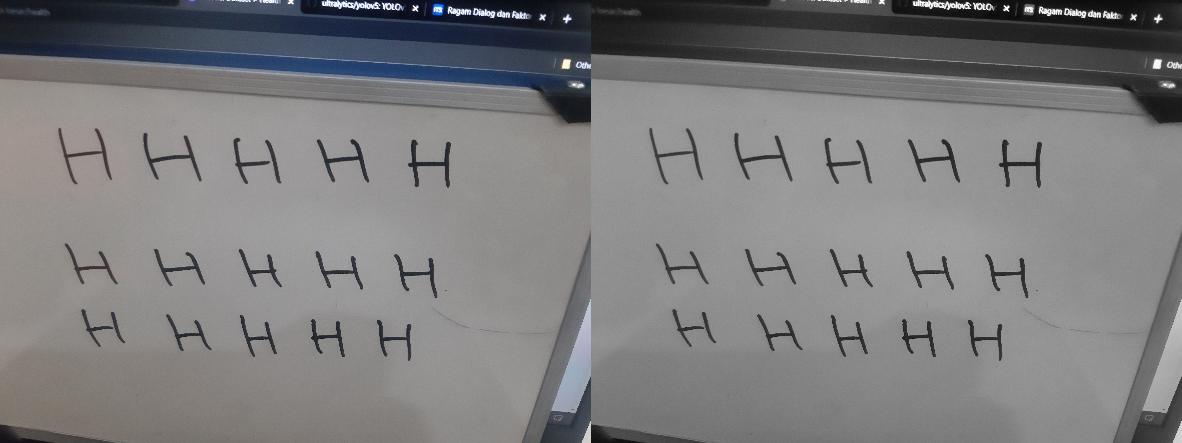
\includegraphics[scale=0.33]{gambar/grayscalling.png}
      \caption{Gambar Sebelum dan Setelah Proses \textit{Grayscalling}}
      \label{fig:grayscallingdataset}
    \end{figure}
  \item \textit{\textbf{Contrast.} Contrast} dilakukan agar tepian-tepian yang ada pada citra dapat lebih terlihat perbedaannya. Jenis \textit{contrast} yang dilakukan yaitu \textit{contrast stretching. Contrast stretching} adalah teknik transformasi citra yaitu meningkatkan kontras dalam citra dengan melakukan \textit{stretch} atau peregangan rentang intensitas nilai untuk menjangkau rentang nilai yang diinginkan.
  % \item \textit{\textbf{Filter Null.}}
  % \item \textit{\textbf{Blur.}}
  % \item \textit{\textbf{Noise.}}
  % \item \textit{\textbf{Bounding Box Rotation.}}
\end{enumerate}

\subsection{Hasil \textit{Training} dan \textit{Validation}}
\label{subsec:hasiltrainvaldata}

% halooooo, chesia was here
Pada tugas akhir ini, \textit{pretrained weight} yang digunakan yaitu YOLOv5s. \textit{pretrained weight} YOLOv5s dipilih karena jika dibandingkan dengan versi lain seperti YOLOv5m, YOLOv5l memiliki hasil yang relatif lebih rendah, namun dengan menggunakan YOLOv5s hasil dapat didapatkan lebih cepat dan juga cocok jika di-\textit{deploy} pada perangkat kecil seperti perangkat \textit{mobile}. Proses \textit{training} data dilakukan setelah proses pengumpulan citra, proses pelabelan, dan pre-proses gambar selesai dilaksanakan. Adapun hasil dari proses \textit{training} ini yaitu berupa model dan detail data angka pada tiap proses pengulangan  (epochs). Detail spesifikasi laptop yang digunakan dalam melakukan proses \textit{training} yaitu sesuai pada Tabel \ref{tb:spesifikasilaptop}, sedangkan detail hyperparameter dan konfigurasi yang digunakan dapat dilihat pada Tabel \ref*{tb:parametertrain} berikut. \par 

% //FIXME: perbarui tabel 
\begin{table}[H]
  \begin{center}
    \begin{tabularx}{0.5\textwidth}{|X<{\centering}|X<{\centering}|}
      \hline
      % \textbf{Parameter}                       & \textbf{Nilai}          \\ \hline
      \textit{Weights}                         & YOLOv5s                 \\ \hline
      \textit{Class Number}                    & 30                      \\ \hline
      Epochs                                   & 50                      \\ \hline
      \textit{Batch-Size}                      & 16                      \\ \hline
      \textit{Image Size}                      & 416                     \\ \hline
      \textit{Learning Rate}                   & 0.01                    \\ \hline
      \textit{Optimizer}                       & SGD                     \\ \hline
    \end{tabularx}
  \end{center}  
  \caption{Detail Hyperparameter yang Digunakan}
  \label{tb:parametertrain}
\end{table}


Proses \textit{training} dilakukan menggunakan dataset \textit{training set}. Setelah dilakukan proses \textit{train} dengan konfigurasi sesuai pada Tabel \ref*{tb:parametertrain}, selanjutnya dilakukan proses \textit{validation.} Pada tahapan \textit{validation} yaitu model diuji dengan menggunakan dataset \textit{validation set} dan kemudian didapatkan hasil \textit{train} berupa \textit{loss, precision, recall, \textnormal{dan} mAP} sesuai Gambar \ref*{fig:trainresult} yaitu: \par

% //FIXME: perbarui tabel
\begin{figure}[H]
  \centering
  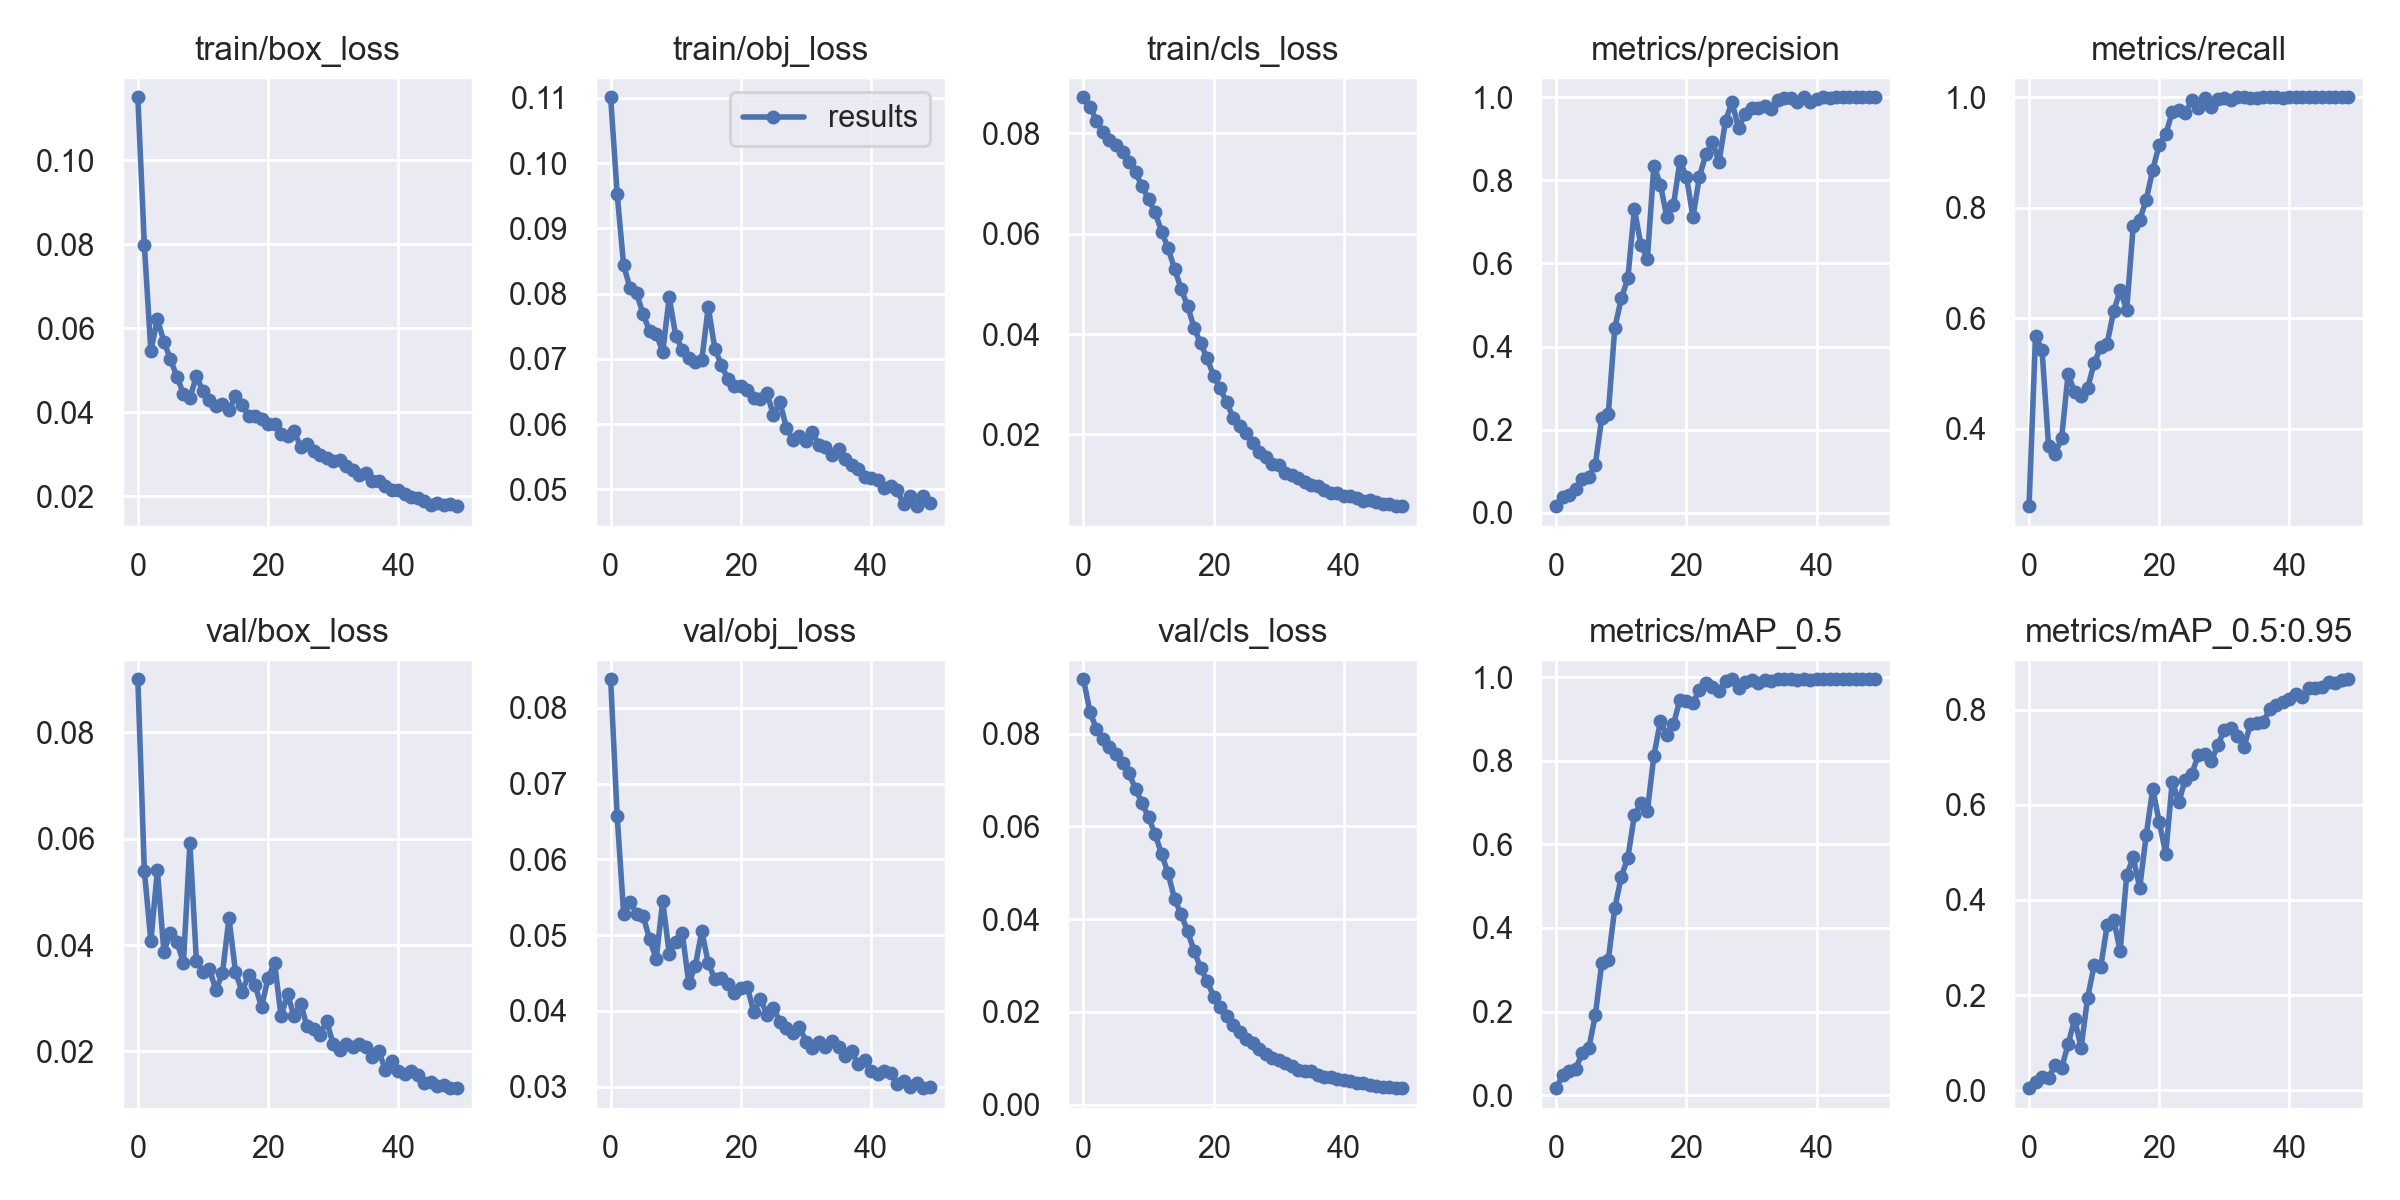
\includegraphics[scale=0.5]{gambar/train_result.png}
  \caption{Hasil Training menggunakan YOLOv5s}
  \label{fig:trainresult}
\end{figure}

\noindent Serta didapatkan detail dari akurasi masing-masing huruf yaitu sebagai berikut: \par

% //FIXME: perbarui tabel
\begin{center}
  \begin{longtable}[c]{|c|c|c|c|c|c|c|}
    \hline
    \textbf{Kelas} & \textbf{Gambar} & \textbf{Jumlah Label} & \textbf{P} & \textbf{R} & \textbf{mAP 0.5} & \textbf{mAP 0.5 0.95} \\ \hline
    \endfirsthead
    %
    \endhead
    %
    *              & 7                          & 105                   & 0.999      & 1          & 0.995            & 0.875                 \\ \hline
    =              & 7                          & 105                   & 0.999      & 1          & 0.995            & 0.907                 \\ \hline
    0              & 7                          & 105                   & 0.999      & 1          & 0.995            & 0.773                 \\ \hline
    1              & 7                          & 105                   & 0.999      & 1          & 0.995            & 0.83                  \\ \hline
    2              & 11                         & 165                   & 1          & 1          & 0.995            & 0.849                 \\ \hline
    3              & 11                         & 165                   & 0.999      & 1          & 0.995            & 0.854                 \\ \hline
    4              & 7                          & 105                   & 0.999      & 1          & 0.995            & 0.895                 \\ \hline
    5              & 7                          & 105                   & 0.999      & 1          & 0.995            & 0.872                 \\ \hline
    6              & 7                          & 105                   & 0.999      & 1          & 0.995            & 0.862                 \\ \hline
    7              & 7                          & 105                   & 1          & 1          & 0.995            & 0.875                 \\ \hline
    8              & 7                          & 105                   & 0.999      & 1          & 0.995            & 0.845                 \\ \hline
    9              & 7                          & 105                   & 0.999      & 1          & 0.995            & 0.859                 \\ \hline
    A              & 7                          & 105                   & 0.999      & 1          & 0.995            & 0.875                 \\ \hline
    B              & 7                          & 105                   & 0.999      & 1          & 0.995            & 0.907                 \\ \hline
    D              & 7                          & 105                   & 0.999      & 1          & 0.995            & 0.83                  \\ \hline
    E              & 11                         & 165                   & 1          & 1          & 0.995            & 0.849                 \\ \hline
    G              & 7                          & 105                   & 0.999      & 1          & 0.995            & 0.895                 \\ \hline
    H              & 7                          & 105                   & 0.999      & 1          & 0.995            & 0.872                 \\ \hline
    I              & 7                          & 105                   & 0.999      & 1          & 0.995            & 0.862                 \\ \hline
    J              & 7                          & 105                   & 1          & 1          & 0.995            & 0.875                 \\ \hline
    K              & 7                          & 105                   & 0.999      & 1          & 0.995            & 0.845                 \\ \hline
    L              & 7                          & 105                   & 0.999      & 1          & 0.995            & 0.859                 \\ \hline
    M              & 11                         & 165                   & 1          & 1          & 0.995            & 0.832                 \\ \hline
    N              & 11                         & 165                   & 1          & 1          & 0.995            & 0.799                 \\ \hline
    P              & 7                          & 105                   & 1          & 1          & 0.995            & 0.824                 \\ \hline
    R              & 7                          & 105                   & 1          & 1          & 0.995            & 0.844                 \\ \hline
    S              & 7                          & 105                   & 1          & 1          & 0.995            & 0.893                 \\ \hline
    T              & 7                          & 105                   & 0.999      & 1          & 0.995            & 0.874                 \\ \hline
    U              & 11                         & 165                   & 0.999      & 1          & 0.995            & 0.844                 \\ \hline
    V              & 11                         & 165                   & 0.999      & 1          & 0.995            & 0.867                 \\ \hline
    W              & 11                         & 165                   & 0.999      & 1          & 0.995            & 0.854                 \\ \hline
    \caption{Hasil Training Perkelas}
    \label{tb:trainperkelas}
  \end{longtable}
\end{center}

% //FIXME: lengkapi berdasarkan data model
Setelah didapatkan hasil model, dilakukan proses pengujian untuk menentukan apakah model tersebut sudah cukup akurat atau masih membutuhkan perbaikan. Pada proses pengujian didapatkan hasil bahwa model 
sementara masih \textit{\textbf{overfit}} dikarenakan walaupun pada hasil \textit{training} memiliki akurasi cukup tinggi, namun ketika dilakukan uji coba menggunakan gambar diluar dataset yag telah disediakan hasilnya masih berantakan. \par
% sudah dapat berfungsi seperti ditunjukkan pada gambar berikut. \par
% //TODO: tambah gambar pas detect model

% \subsection{Hasil \textit{Validation}}
% \label{subsec:hasilvalidation}

\subsection{Hasil Pembuatan Algoritma Konversi Gambar menjadi Teks}
\label{subsec:hasilmembangunmodel}

% //FIXME: lengkapi dengan hasil model
Setelah didapatkan model hasil \textit{training} dan sudah memiliki akurasi cukup untuk dapat melakukan deteksi dengan baik, selanjutnya dilakukan proses pembangunan model konversi gambar menjadi teks. Proses pembangunan model konversi gambar menjadi teks ini diprogram dengan menggunakan bahasa Python. Adapun alur model konversi gambar menjadi teks dimlai dari pengguna melakukan \textit{input} gambar yang ingin dikonversi kedalam program. Setelah gambar dimasukkan kedalam program, gambar tersebut diubah ukurannya menjadi (...), dengan menggunakan \textit{library} opencv. \par

Setelah ukuran gambar disesuaikan, selanjutnya menentukan koordinat seluruh \textit{bounding box} yang tersedia dan terbaca dengan menggunakan model yang telah di\textit{-train} sebelumnya. Setelah koordinat \textit{bounding box} didapat, seluruh \textit{bounding box} yang terbaca dikelompokan berdasarkan jarak antara \textit{bounding box} pertama dengan \textit{bounding box} selanjutnya, jika jarak antaranya memenuhi \textit{threshold} tertentu, maka akan dikelompokan kedalam sebuah List yang sama, dan jika tidak memenuhi maka akan diletakan pada kelompok List berikutnya. Adapun \textit{threshold} yang digunakan yaitu pada koordinat X sebesar (...) dan koordinat Y sebesar (...). Prioritas pengelompokan diatur berdasarkan koordinat Y terlebih dahulu kemudian dilanjutkan dengan koordinat X, hal ini bertujuan agar teks yang ditampilkan berurutan dari baris paling atas lalu bergerak kearah X+ (kanan), dan dilanjut pada baris kedua dan seterusnya. \par

Ketika seluruh \textit{bounding box} telah disortir dan dikelompokkan berdasarkan koordinat X dan Y, proses selanjutnya yaitu seluruh \textit{bounding box} dikembalikan nilainya. Adapun nilai kembalian yang didapatkan dapat ditampilkan dalam gambar langsung ataupun dalam bentuk String. 

\section{Skenario Pengujian}
\label{sec:skenariopengujian}

Pada sub ini dilakukan berbagai skenario pengujian guna mengetahui tingkat kesalahan dan membuka potensi pengembangan penelitian dimasa mendatang serta menarik kesimpulan secara keseluruhan. Secara spesifik, skenario pengujian yang dilakukan yaitu sebagai berikut: \par

\subsection{Pengujian Menggunakan \textit{Pretrained Weight} Model yang Bervariasi}
\label{subsec:pengujianpretrainedweight}

Pada pengujian pertama yaitu pengujian menggunakan \textit{pretrained weight} model yang bervariasi. Tujuan dari pengujian ini yaitu untuk membandingkan performa dan hasil yang didapat dengan performa dan hasil yang didapat dari model lain. Pada pengujian dengan \textit{pretrained weight} model ini menggunakan model YOLOv5n, YOLOv5s, dan YOLOv5m. Pengujian dilaksanakan dengan cara melakukan proses \textit{train} dengan konfigurasi serupa antar parameter dan \textit{hyperparameter.} Pada tiap \textit{pretrained weight} model yang diuji prosesnya diulang sebanyak 2 kali. Dari pengujian pertama ini didapatkan hasil seperti pada Tabel \ref*{tb:variasipretrainedweight} berikut. \par

\begin{center}
  \begin{longtable}[c]{|c|cc|cc|cc|}
    \hline
    \multirow{2}{*}{\textbf{}}                                                         & \multicolumn{2}{c|}{\textbf{YOLOv5n}}  & \multicolumn{2}{c|}{\textbf{YOLOv5s}}  & \multicolumn{2}{c|}{\textbf{YOLOv5m}}  \\ \cline{2-7} 
                                                                                      & \multicolumn{1}{c|}{1}       & 2       & \multicolumn{1}{c|}{1}       & 2       & \multicolumn{1}{c|}{1}       & 2       \\ \hline
    \endfirsthead
    %
    \endhead
    %
    \textit{\textbf{\begin{tabular}[c]{@{}c@{}}Training\\ Box Loss\end{tabular}}}      & \multicolumn{1}{c|}{not yet} & not yet & \multicolumn{1}{c|}{not yet} & not yet & \multicolumn{1}{c|}{not yet} & not yet \\ \hline
    \textit{\textbf{\begin{tabular}[c]{@{}c@{}}Training\\ Object Loss\end{tabular}}}   & \multicolumn{1}{c|}{not yet} & not yet & \multicolumn{1}{c|}{not yet} & not yet & \multicolumn{1}{c|}{not yet} & not yet \\ \hline
    \textit{\textbf{\begin{tabular}[c]{@{}c@{}}Training\\ Class Loss\end{tabular}}}    & \multicolumn{1}{c|}{not yet} & not yet & \multicolumn{1}{c|}{not yet} & not yet & \multicolumn{1}{c|}{not yet} & not yet \\ \hline
    \textit{\textbf{\begin{tabular}[c]{@{}c@{}}Validation\\ Box Loss\end{tabular}}}    & \multicolumn{1}{c|}{not yet} & not yet & \multicolumn{1}{c|}{not yet} & not yet & \multicolumn{1}{c|}{not yet} & not yet \\ \hline
    \textit{\textbf{\begin{tabular}[c]{@{}c@{}}Validation\\ Object Loss\end{tabular}}} & \multicolumn{1}{c|}{not yet} & not yet & \multicolumn{1}{c|}{not yet} & not yet & \multicolumn{1}{c|}{not yet} & not yet \\ \hline
    \textit{\textbf{\begin{tabular}[c]{@{}c@{}}Validation\\ Class Loss\end{tabular}}}  & \multicolumn{1}{c|}{not yet} & not yet & \multicolumn{1}{c|}{not yet} & not yet & \multicolumn{1}{c|}{not yet} & not yet \\ \hline
    \multicolumn{1}{|l|}{\textit{\textbf{Precision}}}                                  & \multicolumn{1}{c|}{not yet} & not yet & \multicolumn{1}{c|}{not yet} & not yet & \multicolumn{1}{c|}{not yet} & not yet \\ \hline
    \multicolumn{1}{|l|}{\textit{\textbf{Recall}}}                                     & \multicolumn{1}{c|}{not yet} & not yet & \multicolumn{1}{c|}{not yet} & not yet & \multicolumn{1}{c|}{not yet} & not yet \\ \hline
    \multicolumn{1}{|l|}{\textbf{mAP}}                                                 & \multicolumn{1}{c|}{not yet} & not yet & \multicolumn{1}{c|}{not yet} & not yet & \multicolumn{1}{c|}{not yet} & not yet \\ \hline
    \caption{Pengujian dengan Variasi Pretrained Weight }
    \label{tb:variasipretrainedweight}\\
  \end{longtable}
\end{center}

% //TODO: tambahin grafik dari tiap training dan tiap jenis model
% Dari tabel berikut dapat terlihat bahwa nilai \textit{loss} terendah yaitu pada model (...) dan nilai precision tertinggi yaitu pada model (...).

\subsection{Pengujian Menggunakan \textit{Input} Citra Tulisan dari Responden Berbeda}
\label{subsec:pengujiancitrabedapenulis}

Pada pengujian kedua yaitu pengujian menggunakan \textit{input} citra tulisan dari penulis berbeda. Tujuan dari pengujian ini yaitu untuk mengetahui akurasi model ketika dihadapkan dengan tulisan dari penulis lain. Hal tersebut diperlukan karena pada proses pembuatan dataset, dataset dibuat berdasarkan gaya penulisan dari 1 orang saja. Pada tahap pengujian ini, penulis meminta responden untuk menuliskan kalimat tertentu kepada beberapa responden dan mengambil citra dari tulisan tersebut untuk kemudian diberikan kepada model. Adapun tulisan yang diberikan sama antar responden dan juga sudut serta jarak pengambilan citra juga disamakan. Perbandingan hasil pembacaan model terhadap citra tulisan dari responden berbeda didapatkan hasil yaitu sebagai berikut.
% //TODO: citra dari 5 orang berbeda

\subsection{Pengujian Menggunakan \textit{Input} Citra dengan Jarak Pengambilan Citra Bervariasi}
\label{subsec:pengujiancitrabedajarak}

Pada pengujian ketiga yaitu pengujian menggunakan \textit{input} citra dengan jarak pengambilan citra yang bervariasi. Tujuan dari pengujian ini yaitu untuk mengetahui akurasi model ketika citra yang akan diberikan diambil dari jarak pengambilan gambar yang berbeda, serta untuk mengetahui pengaruh jarak pengambilan citra dengan performa dari model. Hal tersebut diperlukan karena pada kondisi nyata tidak menutup kemungkinan bahwa citra yang diberikan diambil dari jarak yang cukup jauh ataupun cukup dekat. Adapun pada pengujian kali ini, variasi yang digunakan yaitu pengambilan citra pada jarak kisaran 20cm, kisaran 30cm, dan kisaran 40cm. Perbandingan hasil pembacaan model terhadap citra tulisan dari jarak pengambilan bervariasi didapatkan hasil yaitu seperti pada Gambar \ref*{fig:citra20cm}, Gambar \ref*{fig:citra30cm}, dan Gambar \ref*{fig:citra40cm} berikut.

% //FIXME: ganti gambar, versi terang dari 2 konten isi berbeda (sama penulis, beda konten)
% 20cm
\begin{figure}[H]
  \begin{subfigure}{.5\textwidth}
    \centering
    \captionsetup{width=.8\linewidth}
    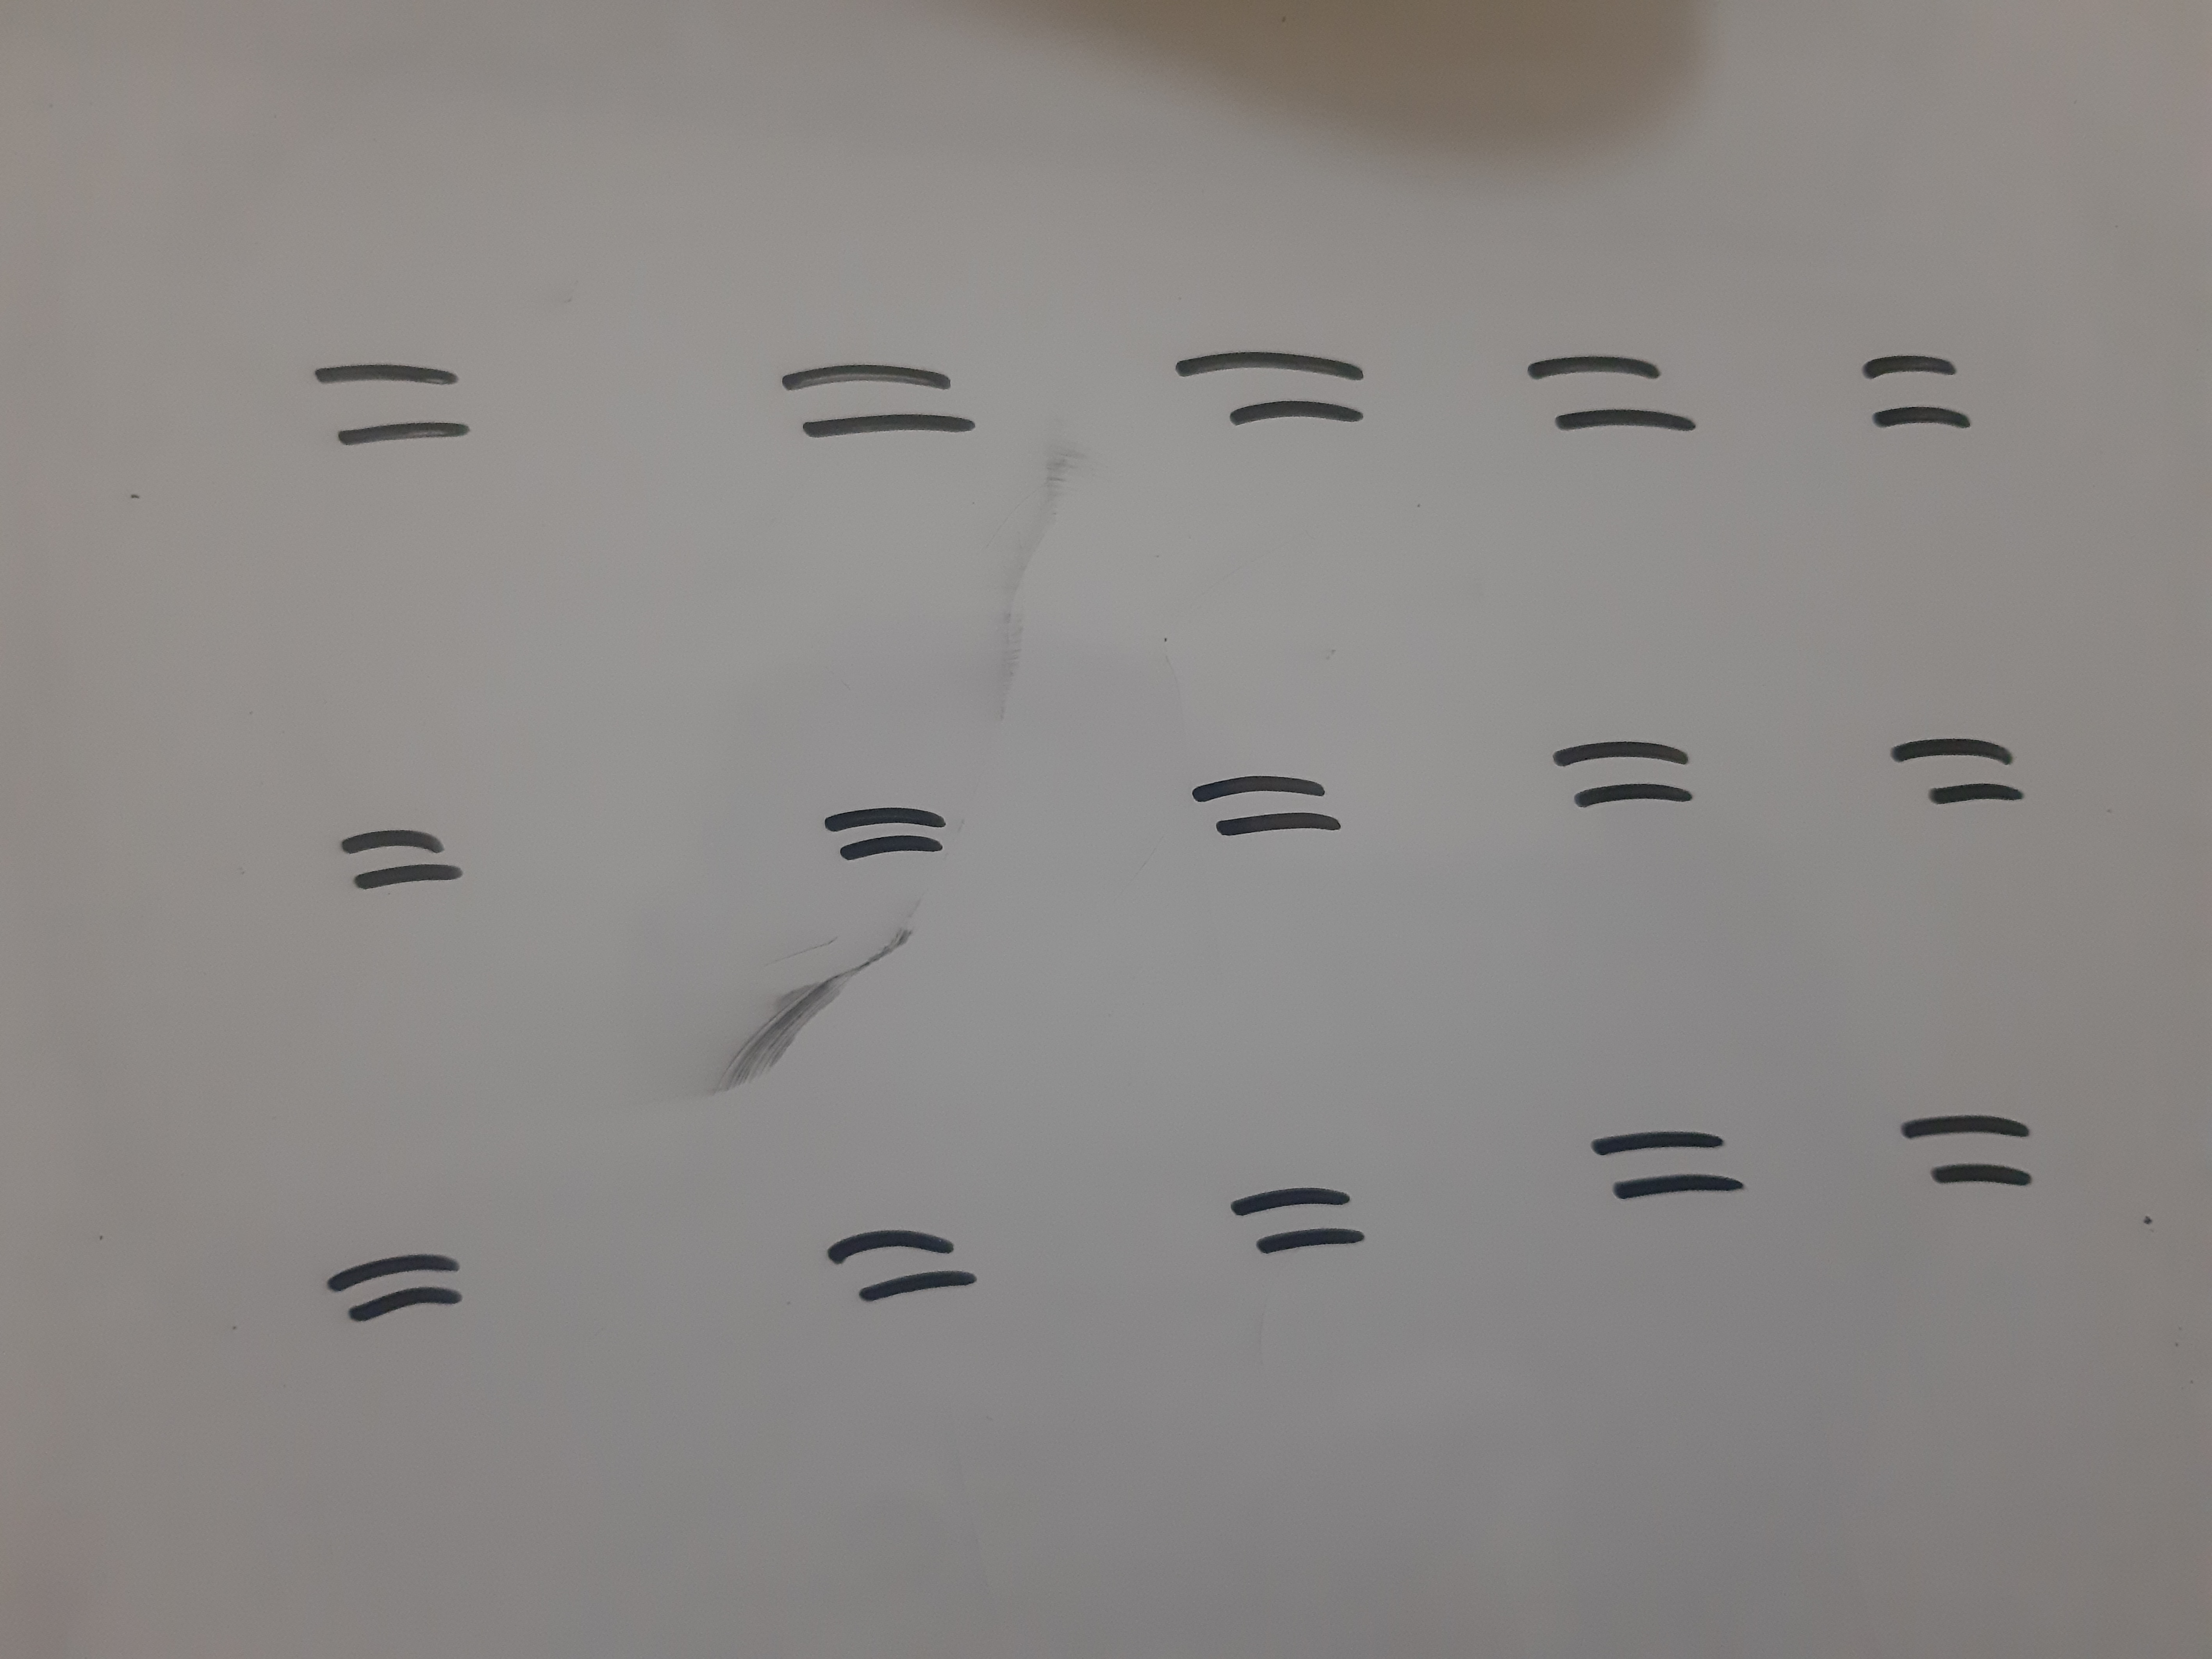
\includegraphics[width=.85\linewidth]{gambar/pengambilan_citra_terang.jpg}
    \caption{Sampel 1, Pengambilan Citra Jarak 20 Cm}
    \label{fig:citra120cm}
  \end{subfigure}%
  \begin{subfigure}{.5\textwidth}
    \centering
    \captionsetup{width=.8\linewidth}
    \includegraphics[width=.85\linewidth]{gambar/pengambilan_citra_gelap.jpg}
    \caption{Sampel 2, Pengambilan Citra Jarak 20 Cm}
    \label{fig:citra220cm}
  \end{subfigure}
  \caption{Pengambilan Citra Jarak 20 Cm}
  \label{fig:citra20cm}
\end{figure}

% 30cm
\begin{figure}[H]
  \begin{subfigure}{.5\textwidth}
    \centering
    \captionsetup{width=.8\linewidth}
    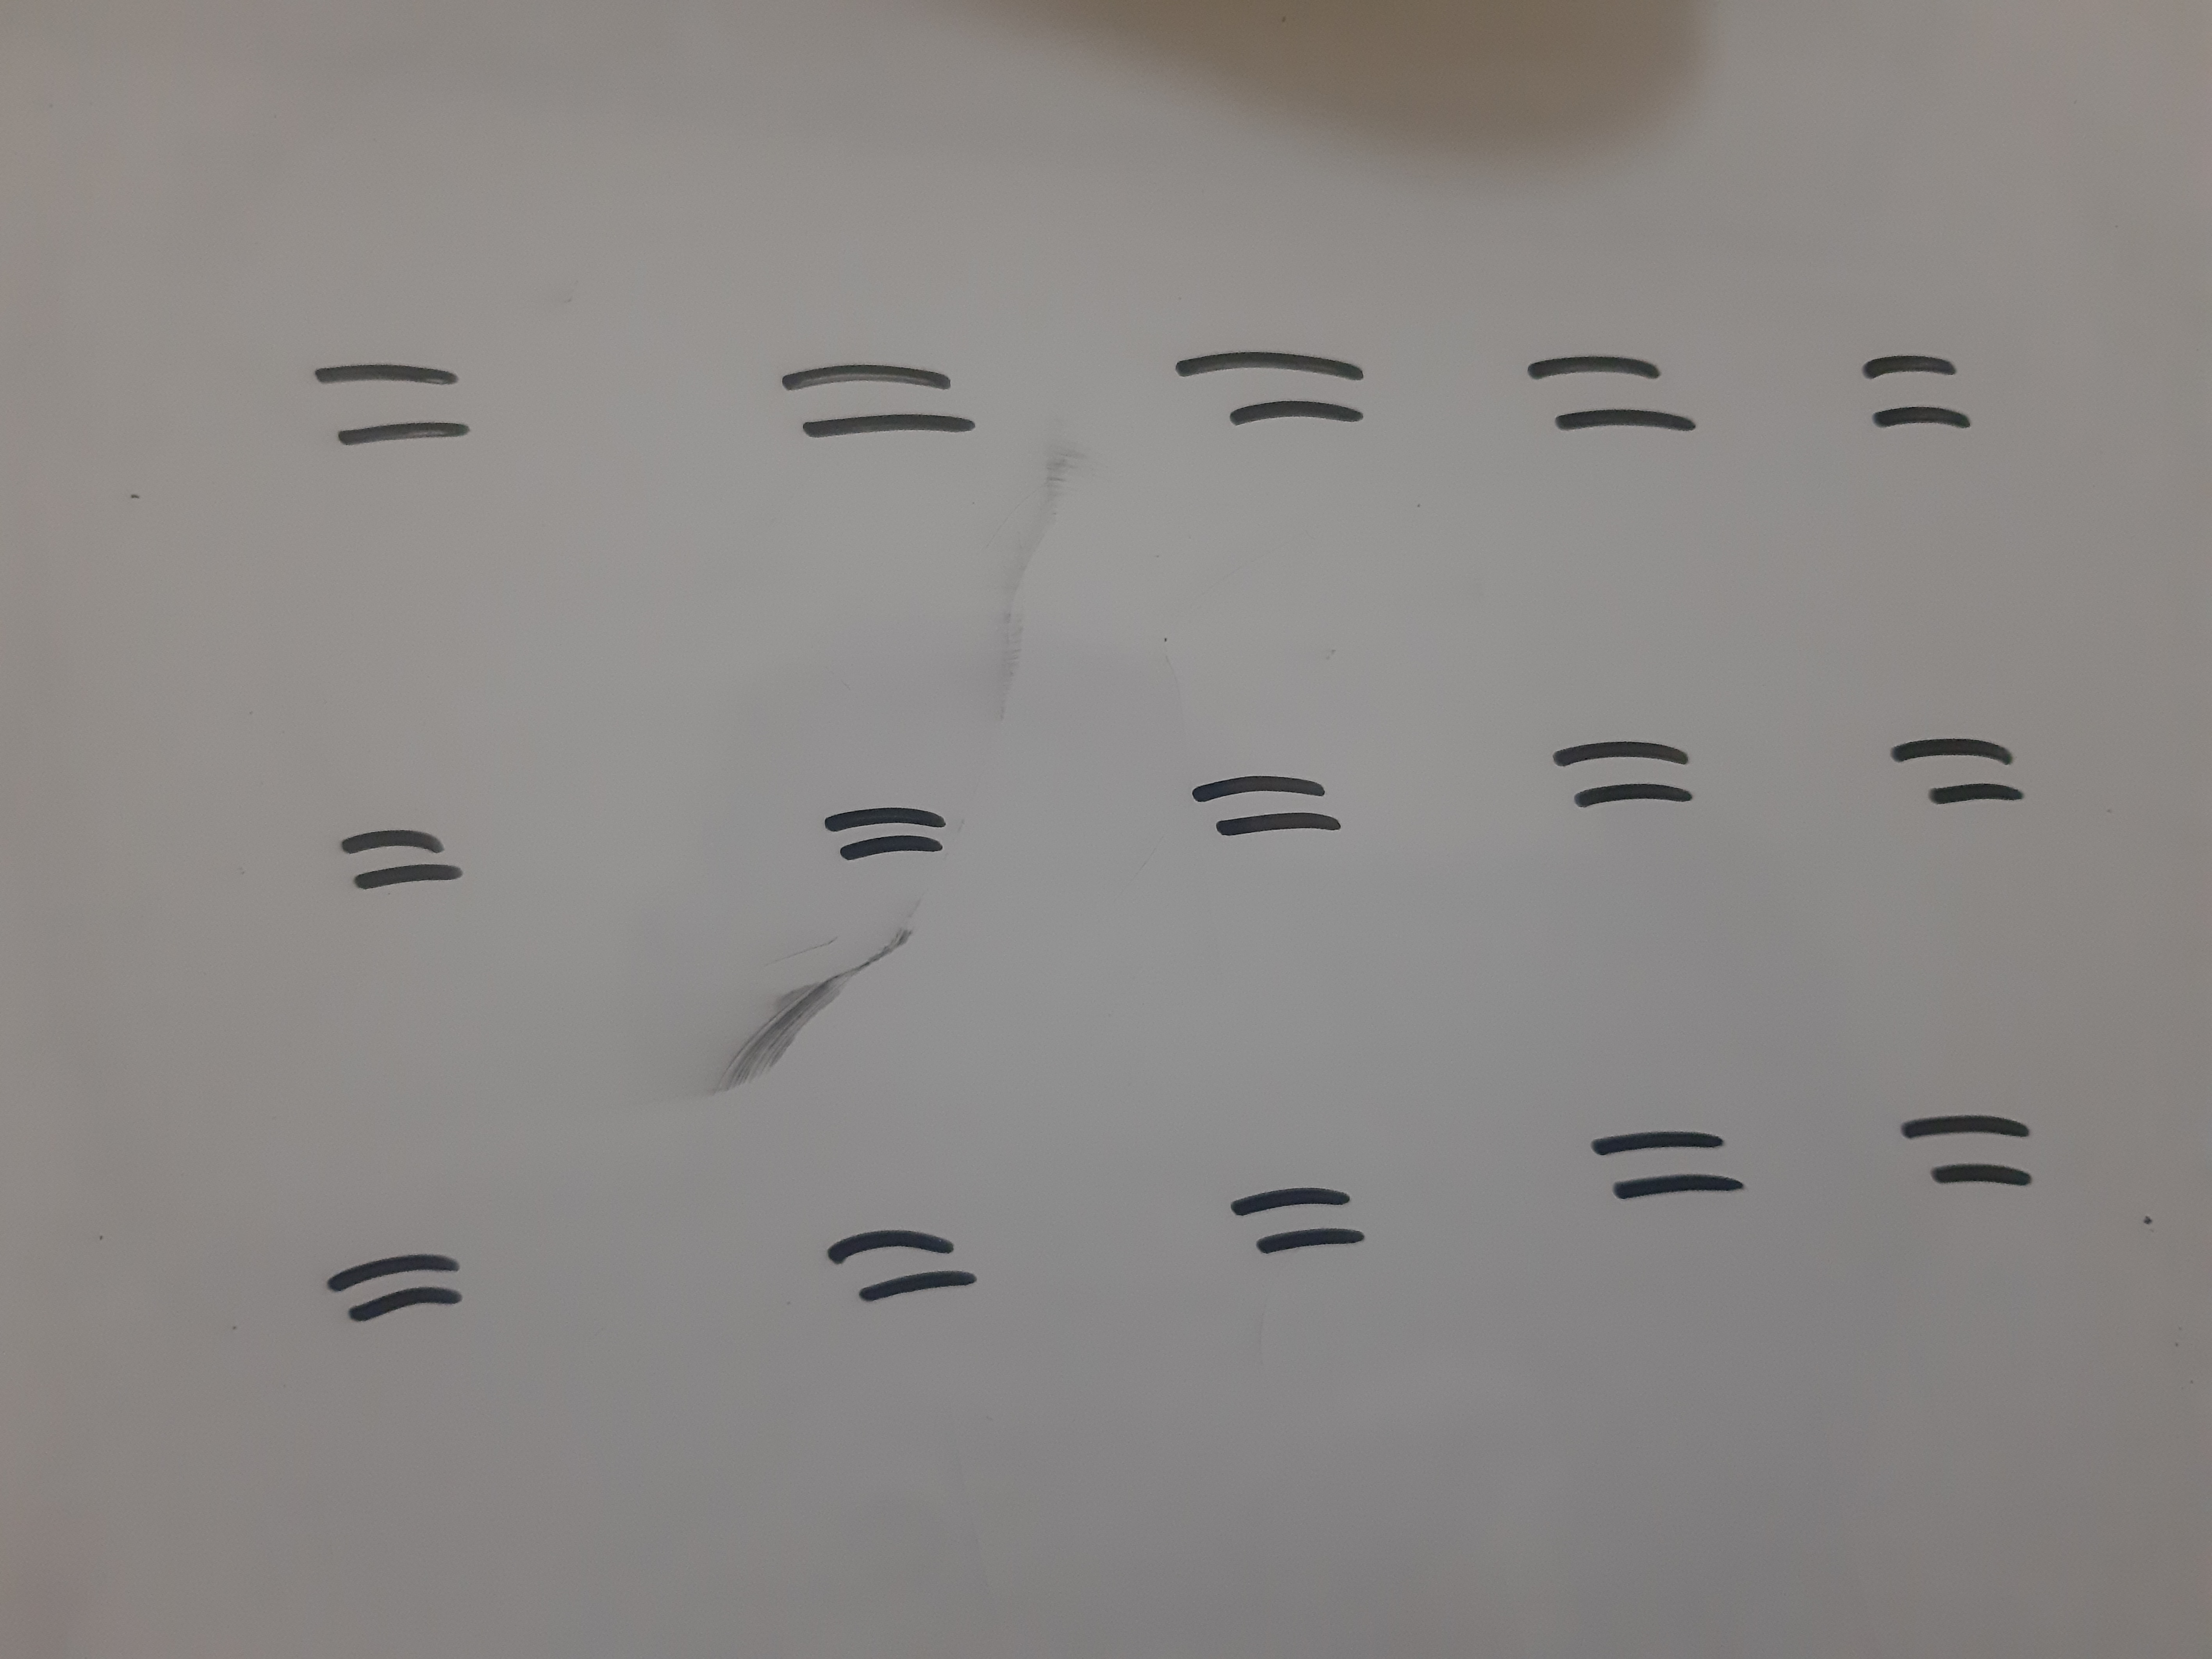
\includegraphics[width=.85\linewidth]{gambar/pengambilan_citra_terang.jpg}
    \caption{Sampel 1, Pengambilan Citra Jarak 30 Cm}
    \label{fig:citra130cm}
  \end{subfigure}%
  \begin{subfigure}{.5\textwidth}
    \centering
    \captionsetup{width=.8\linewidth}
    \includegraphics[width=.85\linewidth]{gambar/pengambilan_citra_gelap.jpg}
    \caption{Sampel 2, Pengambilan Citra Jarak 30 Cm}
    \label{fig:citra230cm}
  \end{subfigure}
  \caption{Pengambilan Citra Jarak 30 Cm}
  \label{fig:citra30cm}
\end{figure}

% 40cm
\begin{figure}[H]
  \begin{subfigure}{.5\textwidth}
    \centering
    \captionsetup{width=.8\linewidth}
    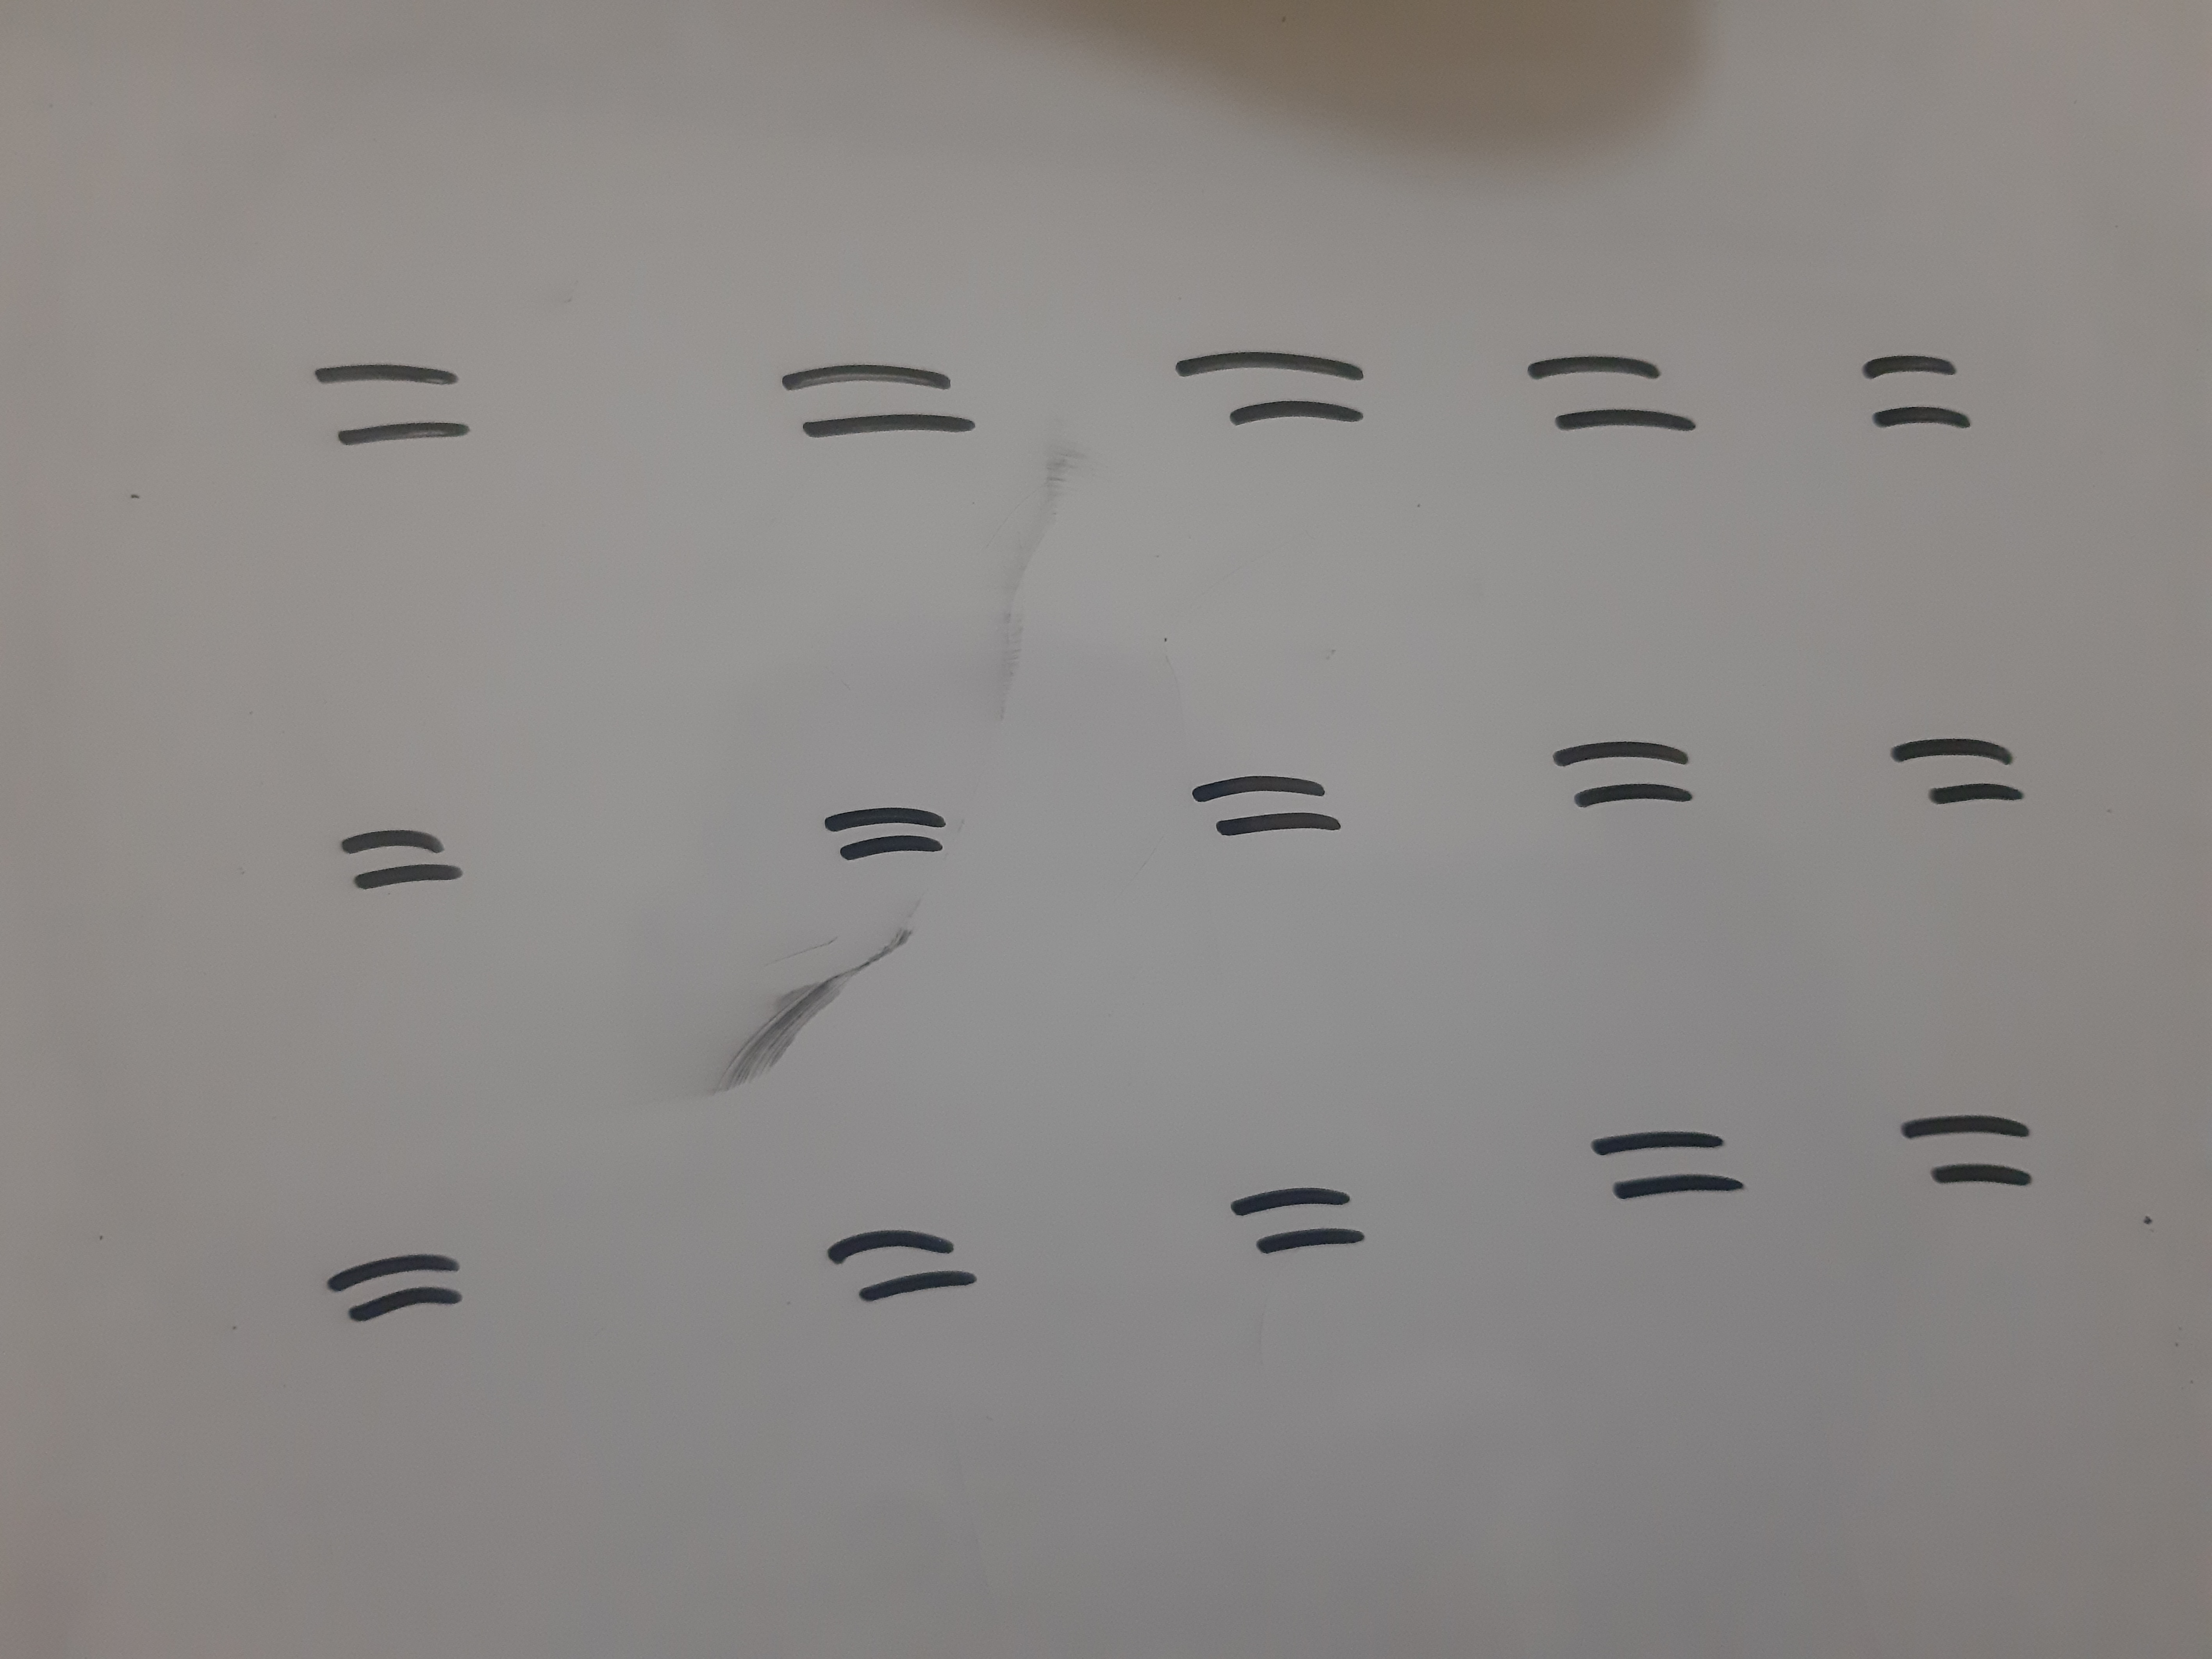
\includegraphics[width=.85\linewidth]{gambar/pengambilan_citra_terang.jpg}
    \caption{Sampel 1, Pengambilan Citra Jarak 40 Cm}
    \label{fig:citra140cm}
  \end{subfigure}%
  \begin{subfigure}{.5\textwidth}
    \centering
    \captionsetup{width=.8\linewidth}
    \includegraphics[width=.85\linewidth]{gambar/pengambilan_citra_gelap.jpg}
    \caption{Sampel 2, Pengambilan Citra Jarak 40 Cm}
    \label{fig:citra240cm}
  \end{subfigure}
  \caption{Pengambilan Citra Jarak 40 Cm}
  \label{fig:citra40cm}
\end{figure}

\subsection{Pengujian Menggunakan \textit{Input} Citra dengan Pencahayaan Pengambilan Citra Bervariasi}
\label{subsec:pengujiancitrabedaintensitas}

Pada pengujian keempat yaitu pengujian dengan menggunakan \textit{input} citra dengan pencahayaan pengambilan citra bervariasi. Tujuan dari pengujian ini yaitu untuk mengetahui pengaruh akurasi model ketika citra yang akan diberikan diambil dengan kondisi pencahayaan yang beragam, serta untuk mengetahui pengaruh pencahayaan dalam pengambilan citra dengan performa dari model. Adapun pada pengujian ini, pengaturan pencahayaan diatur menggunakan fungsi \textit{apperture} yang ada pada kamera. \textit{Apperture} pada kamera untuk pengambilan citra diatur dengan kondisi yaitu kondisi \textit{default} dan juga dengan kondisi \textit{exposure} -1.5 \textit{steps.} Perbandingan hasil pembacaan model terhadap variasi pencahayaan didapatkan hasil yaitu seperti pada Gambar \ref*{fig:citracahayavariasi1}, Gambar \ref*{fig:citracahayavariasi2}, dan Gambar \ref*{fig:citracahayavariasi3} berikut.
% exposure 0 dan -1.5
% //FIXME: ganti gambar, versi terang n gelap dari 2 konten isi sama (sama penulis, sama konten)

% pengujian 1
\begin{figure}[H]
  \begin{subfigure}{.5\textwidth}
    \centering
    \captionsetup{width=.8\linewidth}
    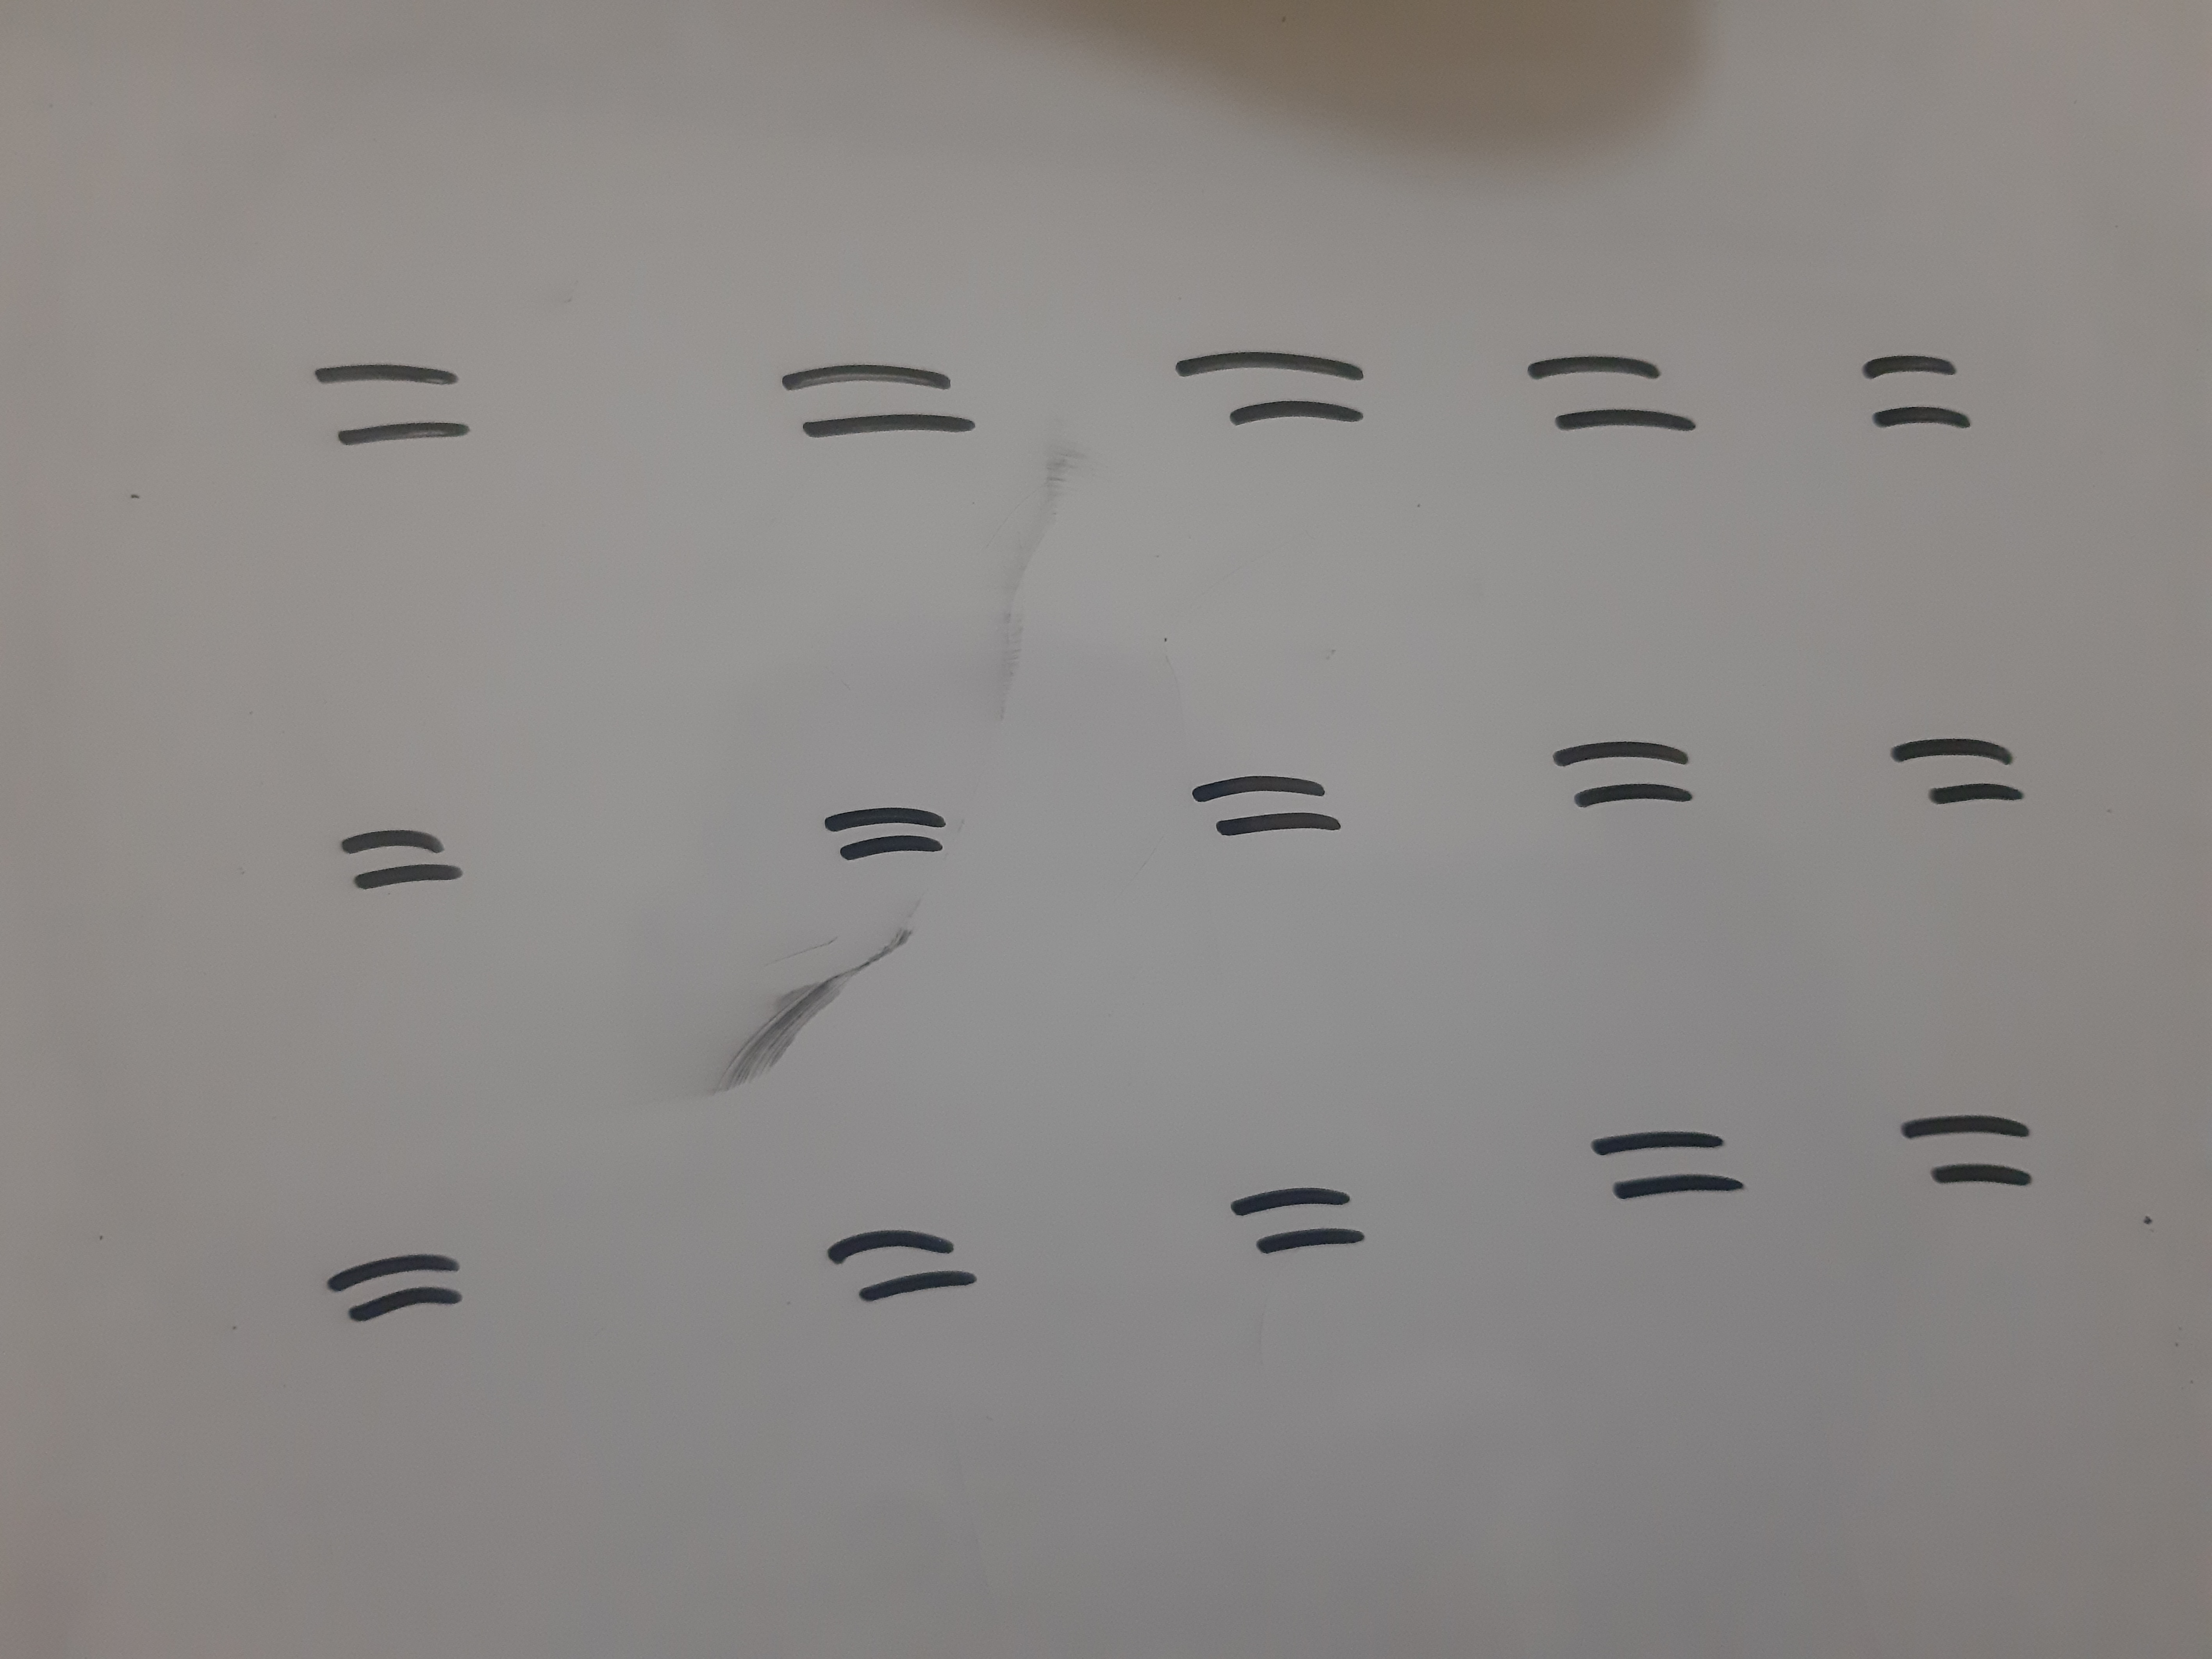
\includegraphics[width=.85\linewidth]{gambar/pengambilan_citra_terang.jpg}
    \caption{Pengambilan Citra Pencahayaan Normal}
    \label{fig:1citracahaya0}
  \end{subfigure}%
  \begin{subfigure}{.5\textwidth}
    \centering
    \captionsetup{width=.8\linewidth}
    \includegraphics[width=.85\linewidth]{gambar/pengambilan_citra_gelap.jpg}
    \caption{Pengambilan Citra Pencahayaan \textit{Apperture} -1 \textit{Steps.}}
    \label{fig:1citracahayamin10}
  \end{subfigure}
  \caption{Pengujian 1, Citra dengan Pencahayaan Berbeda}
  \label{fig:citracahayavariasi1}
\end{figure}

% pengujian 2
\begin{figure}[H]
  \begin{subfigure}{.5\textwidth}
    \centering
    \captionsetup{width=.8\linewidth}
    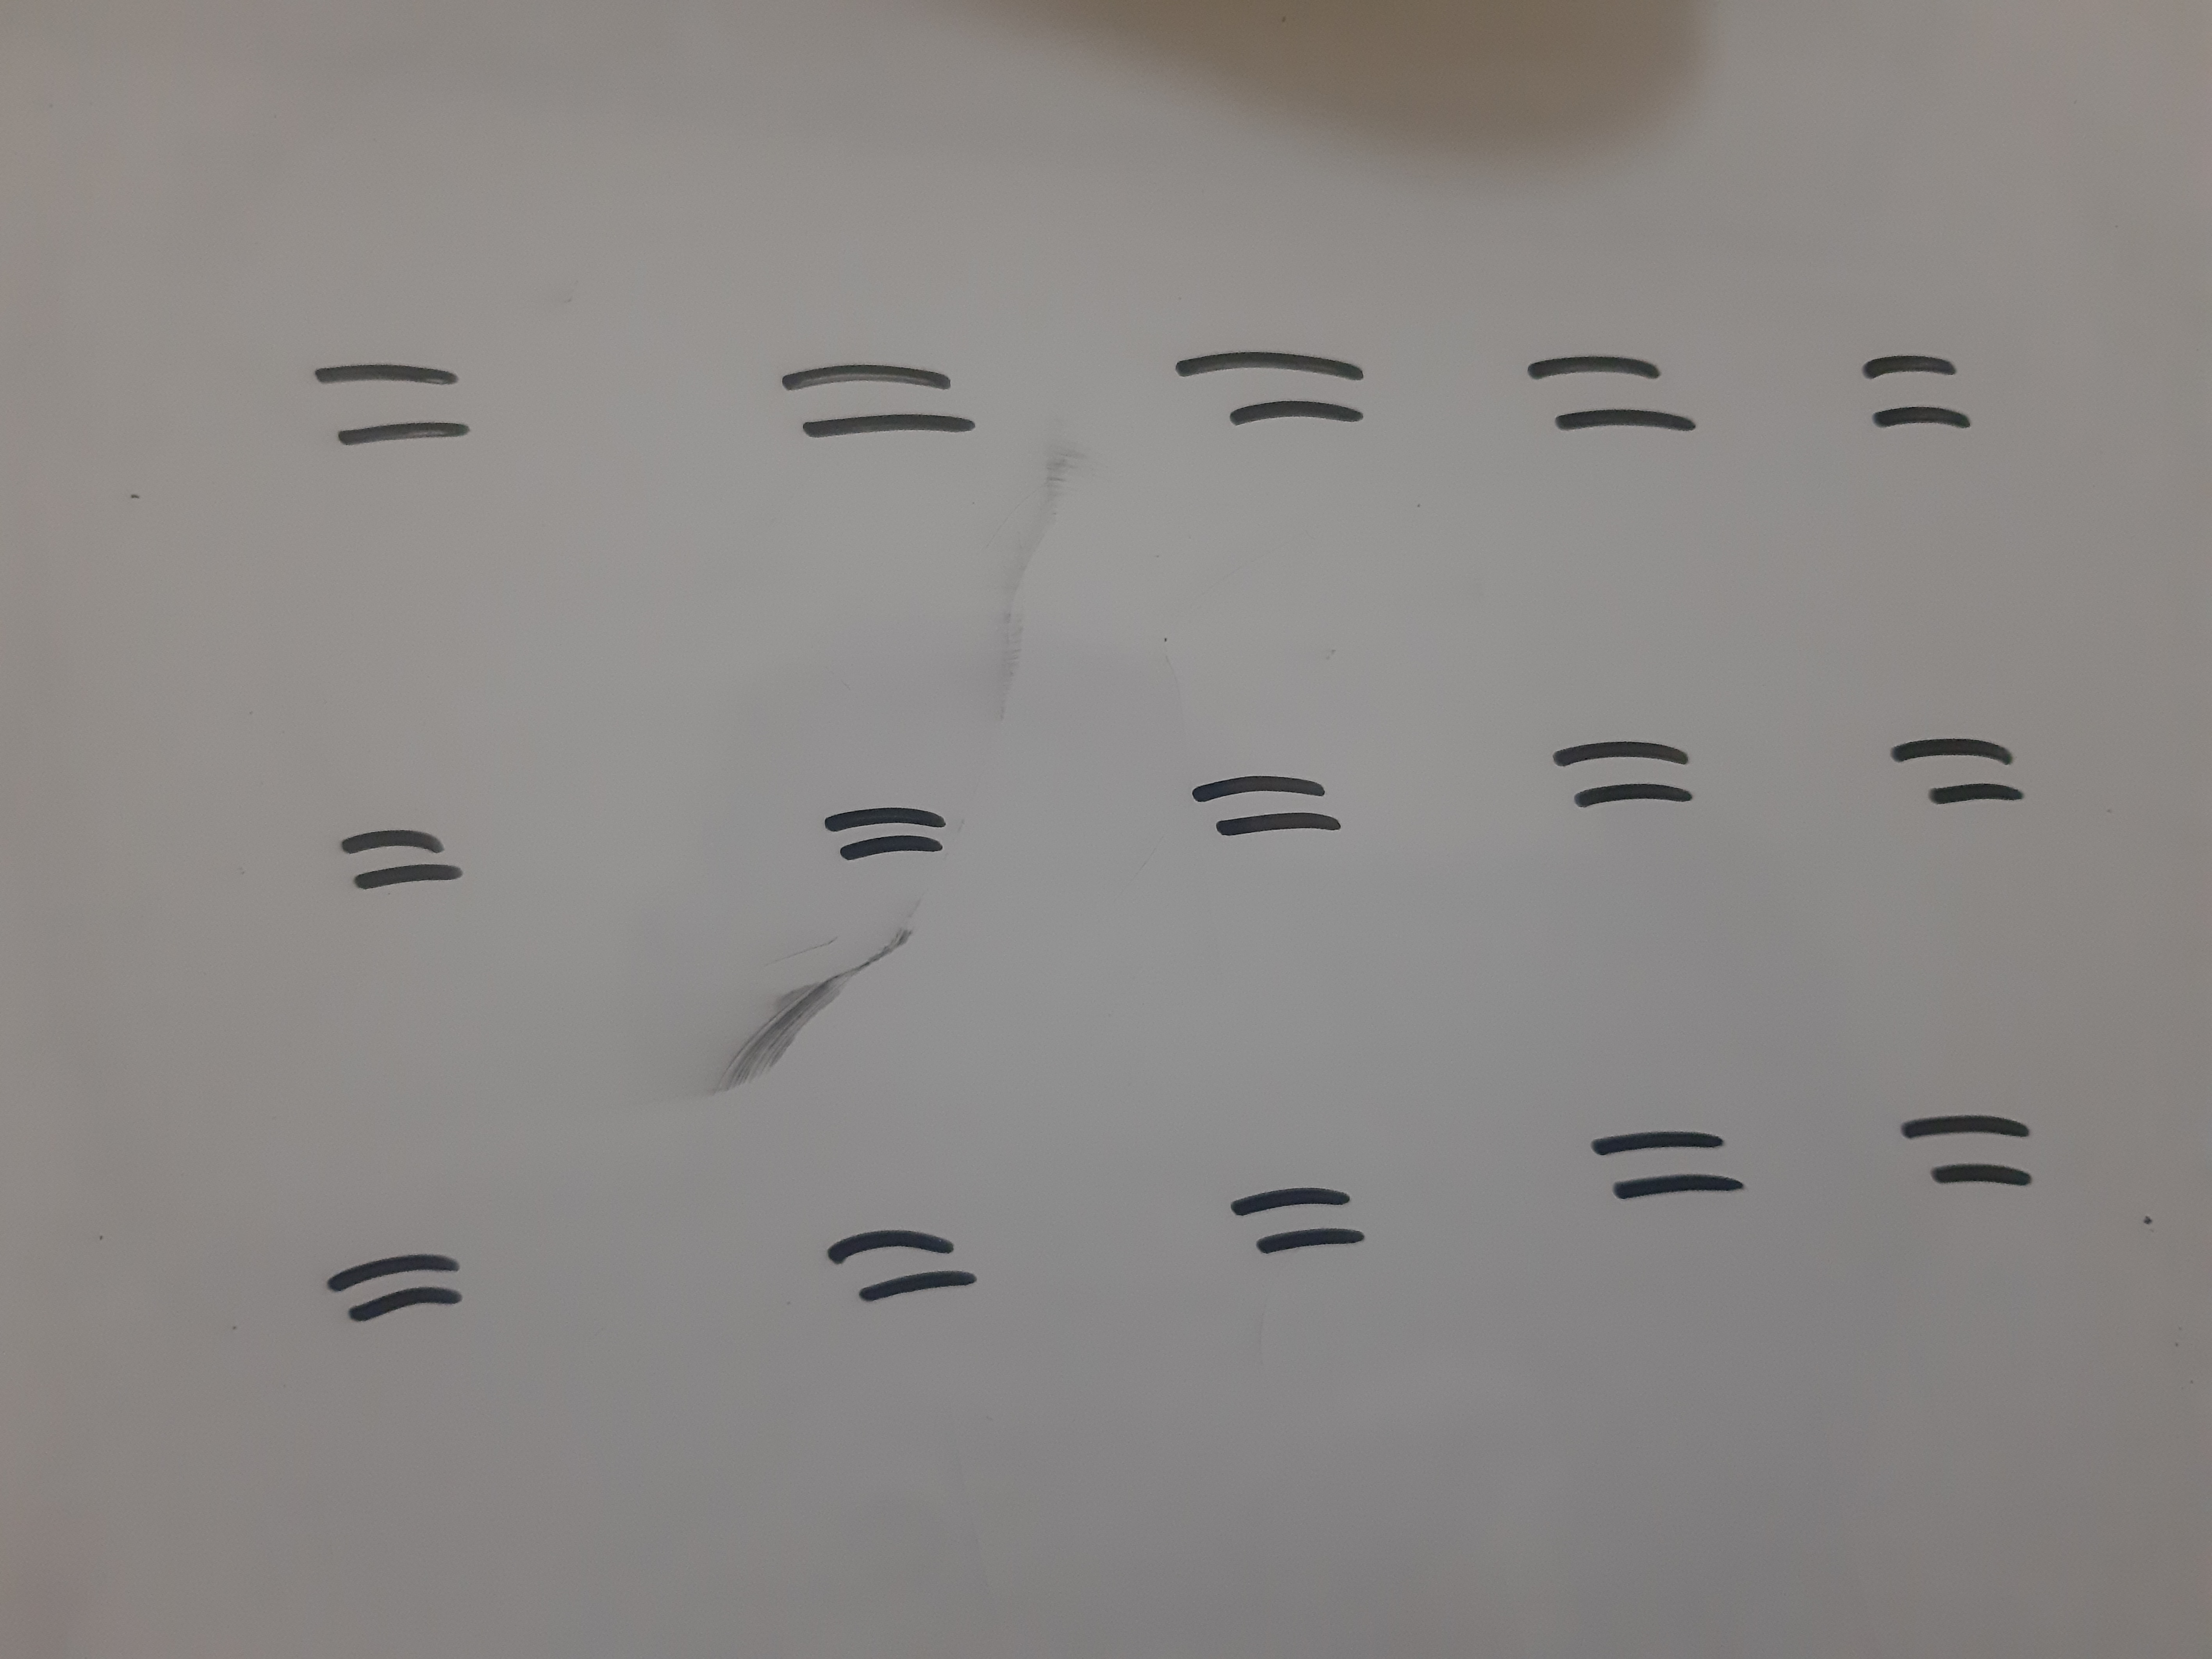
\includegraphics[width=.85\linewidth]{gambar/pengambilan_citra_terang.jpg}
    \caption{Pengambilan Citra Pencahayaan Normal}
    \label{fig:2citracahaya0}
  \end{subfigure}%
  \begin{subfigure}{.5\textwidth}
    \centering
    \captionsetup{width=.8\linewidth}
    \includegraphics[width=.85\linewidth]{gambar/pengambilan_citra_gelap.jpg}
    \caption{Pengambilan Citra Pencahayaan \textit{Apperture} -1 \textit{Steps.}}
    \label{fig:2citracahayamin10}
  \end{subfigure}
  \caption{Pengujian 2, Citra dengan Pencahayaan Berbeda}
  \label{fig:citracahayavariasi2}
\end{figure}

% pengujian 3
\begin{figure}[H]
  \begin{subfigure}{.5\textwidth}
    \centering
    \captionsetup{width=.8\linewidth}
    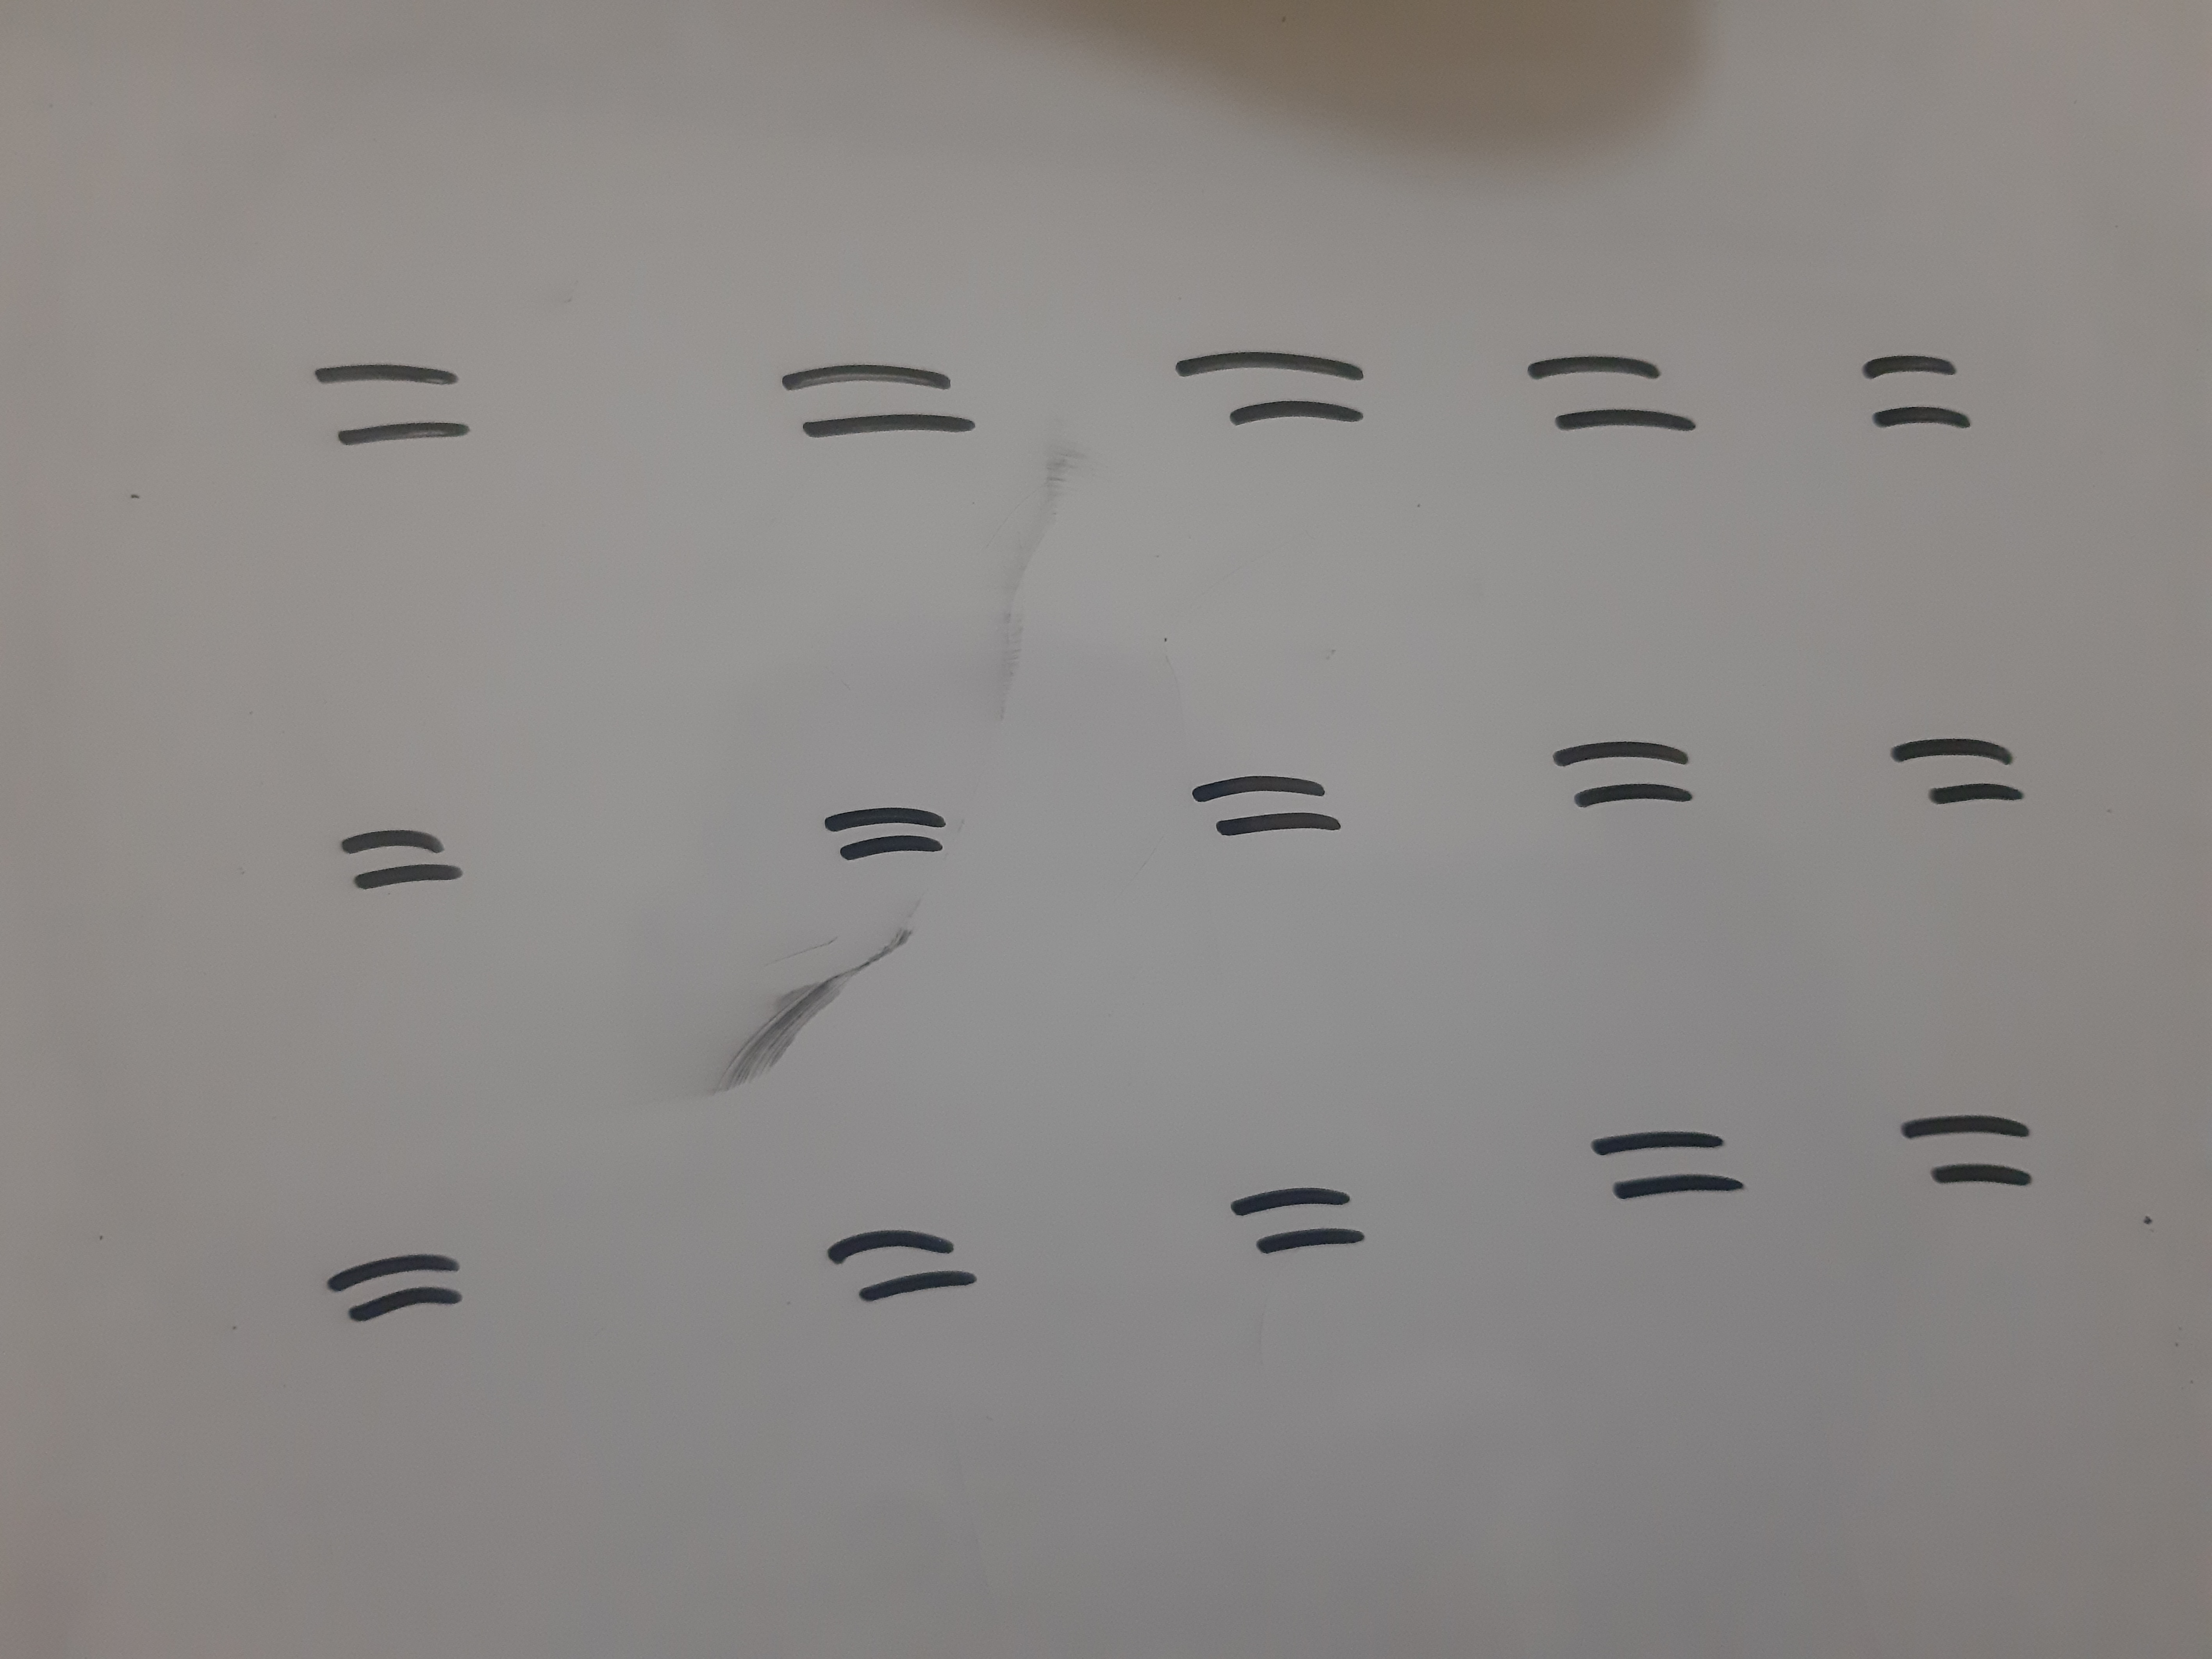
\includegraphics[width=.85\linewidth]{gambar/pengambilan_citra_terang.jpg}
    \caption{Pengambilan Citra Pencahayaan Normal}
    \label{fig:3citracahaya0}
  \end{subfigure}%
  \begin{subfigure}{.5\textwidth}
    \centering
    \captionsetup{width=.8\linewidth}
    \includegraphics[width=.85\linewidth]{gambar/pengambilan_citra_gelap.jpg}
    \caption{Pengambilan Citra Pencahayaan \textit{Apperture} -1 \textit{Steps.}}
    \label{fig:3citracahayamin10}
  \end{subfigure}
  \caption{Pengujian 3, Citra dengan Pencahayaan Berbeda}
  \label{fig:citracahayavariasi3}
\end{figure}

% \section{Evaluasi Pengujian}
% \label{sec:analisispengujian}

% % //FIXME: gatau harus dipakai atau tidak
% \subsection{Evaluasi Pengujian \textit{Training}}
% \label{subsec:evaluasitraining}

% \subsection{Evaluasi Pengujian Menggunakan \textit{Pretrained Weight} Berbeda}
% \label{subsec:evaluasipengujianpretrainedweight}

% \subsection{Evaluasi Pengujian Menggunakan \textit{Input} Citra Tulisan dari Penulis Berbeda}
% \label{subsec:evaluasipengujiancitrabedapenulis}

% \subsection{Evaluasi Pengujian Menggunakan \textit{Input} Citra dengan Jarak Pengambilan Citra Bervariasi}
% \label{subsec:evaluasipengujiancitrabedajarak}

% \subsection{Evaluasi Pengujian Menggunakan \textit{Input} Citra dengan Intensitas Pengambilan Citra Bervariasi}
% \label{subsec:evaluasipengujiancitrabedaintensitas}

  \cleardoublepage

  % Bab 5 penutup
  \chapter{PENUTUP}
\label{chap:penutup}

Pada bab ini akan dipaparkan kesimpulan dari hasil pengujian yang akan menjadi jawaban dari permasalahan yang diangkat oleh pelaksanaan tugas akhir ini. Selain itu juga, dipaparkan saran mengenai hal yang dapat dilakukan untuk mengembangkan penelitian ini kedepannya.
% Ubah bagian-bagian berikut dengan isi dari penutup

\section{Kesimpulan}
\label{sec:kesimpulan}

Berdasarkan hasil pelaksanaan metodologi dan skenario pengujian, dapat diambil beberapa kesimpulan sebagai berikut:
\begin{enumerate}[nolistsep]
    \item Arsitektur YOLO dapat digunakan untuk proses terdeteksi tulisan tangan pada papan tulis. Adapun hasil model dengan menggunakan YOLOv5s didapatkan nilai mAP sebesar 0.828.
    \item Dari pengujian variasi \textit{pretrained weight,} didapatkan hasil bahwa semakin kompleks varian yang digunakan maka hasil yang didapatkan akan semakin baik, namun waktu yang dibutuhkan dalam proses pembuatan model akan memakan waktu lebih lama juga. Dalam hal ini proses train menggunakan YOLOv5s dengan dataset yang telah dibuat membutuhkan waktu 4 jam untuk proses train sedangkan YOLOv5m dengan pengaturan yang sama membutuhkan waktu 8 jam untuk proses train.
    \item Dari pengujian dengan variasi jarak, didapatkan hasil bahwa jarak pengambilan citra memiliki pengaruh penting, karena jika objek citra diambil pada jarak yang terlalu dekat atau terlalu jauh maka hasilnya akan semakin tidak optimal. Adapun pada pelaksanaan tugas akhir ini, hasil optimal didapatkan pada pengambilan citra dengan jarak kisaran 20cm.
    \item Dari pengujian dengan variasi intensitas cahaya, didapatkan hasil bahwa intensitas cahaya dalam pengambilan citra memiliki peran penting, karena pada dasarnya \textit{object detection deep learning} memanfaatkan \textit{edge detection} sehingga jika pencahayaan terlalu tinggi ataupun terlalu rendah mengakibatkan tingkat kontras antara objek dan non objek tidak memiliki kontras yang tinggi. Adapun pada penelitian tugas akhir ini hasil optimal didapatkan ketika pencahayaan dalam kondisi sedikit lebih gelap (kondisi \textit{apperture -1 steps}).
\end{enumerate}

\section{Saran}
\label{chap:saran}

Untuk keperluan pengembangan dari penelitian ini, saran yang dapat diambil yaitu:
\begin{enumerate}[nolistsep]
    \item Menambahkan dataset untuk keperluan \textit{train, validation \textnormal{ataupun} testing}, terutama dengan variasi penulis berbeda mengingat hasil yang didapatkan ketika menggunakan data dari responden memiliki hasil pembacaan lebih rendah.
\end{enumerate}

% Untuk pengembangan lebih lanjut pada \lipsum[1][1-3] antara lain:

% \begin{enumerate}[nolistsep]

%   \item Memperbaiki \lipsum[2][1-3]

%   \item \lipsum[2][4-6]

%   \item \lipsum[2][7-10]

% \end{enumerate}

  \cleardoublepage

  % Daftar pustaka
  \renewcommand\bibname{DAFTAR PUSTAKA}
  \addcontentsline{toc}{chapter}{\bibname}
  \bibliographystyle{unsrtnat}
  \bibliography{pustaka/pustaka.bib}
  \cleardoublepage

  % Biografi penulis
  \begin{center}
  \Large
  \textbf{BIOGRAFI PENULIS}
\end{center}

\addcontentsline{toc}{chapter}{BIOGRAFI PENULIS}

\vspace{2ex}

\begin{wrapfigure}{L}{0.3\textwidth}
  \centering
  \vspace{-3ex}
  % Ubah file gambar berikut dengan file foto dari mahasiswa
  
\includegraphics[width=0.3\textwidth]{gambar/elon.jpg}
  \vspace{-4ex}
\end{wrapfigure}

% Ubah kalimat berikut dengan biografi dari mahasiswa
Elon Reeve Musk, lahir pada \lipsum[1]

\lipsum[2]

  \cleardoublepage

\end{document}
